%%% Local Variables:
%%% TeX-master: "developer.tex"
%%% ispell-local-dictionary: "english"
%%% End:

\chapter{Advanced Plug-in Development}\label{chap:advance}
\lstset{language=Ocaml} %% makes Ocaml the default language for listings, eg. \lstinline.

This chapter details how to use services provided by \framac in order to be
fully operational with the development of plug-ins. Each section describes
technical points a developer should be aware of. Otherwise,
one could find oneself in one or more of the following situations
\footnote{It
  is fortunately quite difficult (but not impossible) to fall into the worst
  situation by mistake if you are not a kernel developer.}
(from bad to worse):
\begin{enumerate}
\item reinventing the (\framac) wheel;
\item being unable to do some specific things (\eg saving
  results\index{Saving} of an analysis on disk, see
  Section~\ref{proj:states});
\item introducing bugs in his/her code;
\item introducing bugs in other plug-ins using his/her code;
\item breaking the kernel consistency\index{Consistency} and so potentially
  breaking all \framac plug-ins (\eg if s/he modifies the
  AST\index{AST!Modification} without changing project\index{Project}, see
  Section~\ref{proj:use}).
\end{enumerate}

In this chapter, we suppose that the reader is able to write a minimal plug-in
like \texttt{hello}\index{Hello} described in chapter~\ref{chap:tutorial} and
knows about the software architecture of \framac (chapter~\ref{chap:archi}). Moreover
plug-in development requires the use of advanced features of
\caml (module system, classes and objects, \emph{etc}).
Plug-in development also requires some familiarity with the Dune build system.

Note that the following subsections can be read in no particular
order: their contents are indeed quite independent from one another even if
there are references from one section to another one.

\section{Plug-in dependencies}\label{adv:dependencies}

\begin{target}standard plug-in developers.\end{target}

\begin{prereq}
  Basic knowledge of the Dune build system.
\end{prereq}

Some plug-ins only depend on the \framac kernel, and in this case, require no
special configuration. However, many plug-ins depend either on other \framac
plug-ins, or on external libraries, tools and components. In both cases, it is
important to specify such dependencies, to avoid the user trying and failing
to compile or run your plug-in.

Plug-in dependencies are usually defined in the plug-in's \verb|dune| file.
There are mainly two kinds of dependencies: {\em mandatory} and {\em optional}.
Mandatory dependencies are necessary for the plug-in to run {\em at all}, and
their absence means the plug-in must be disabled. Optional dependencies do not
prevent compilation and usage of the plug-in, but it may work less efficiently,
precisely, or fail when specific features are requested.

\begin{important}
  Plug-in developers must ensure that optional dependencies are tested for
  their absence and dealt with gracefully; a plug-in must {\em not} crash when
  optional dependencies are missing.
\end{important}

Most dependencies (OCaml library dependencies, such as other plug-ins or OCaml
modules) are specified using Dune's \verb|library| stanza%
\footnote{Full documentation about Dune's \texttt|library| stanza is available
at \url{https://dune.readthedocs.io/en/stable/concepts.html\#library-deps}}.
As is often the case, examples are very instructive; here is an example of
mandatory dependencies from the \textsf{Dive} plug-in's \verb|dune| file:

\begin{lstlisting}[language=Dune]
(library
  [...]
  (libraries frama-c.kernel frama-c-studia.core frama-c-server.core)
)
\end{lstlisting}

The \verb|libraries| field contains \verb|frama-c.kernel| (essential for all
plug-ins), but also \verb|frama-c-studia.core| and \verb|frama-c-server.core|,
meaning this plug-in requires both the \textsf{Studia} and \textsf{Server}
plug-ins to be enabled. If any of them is disabled (either due to
missing dependencies, or as a result of a user request), then \textsf{Dive}
will also be disabled.

{\em Note: to explicitly disable a plug-in, use the
  \verb|dev/disable-plugins.sh| script.}

Note that OCaml libraries can also be specified, e.g. adding \verb|zarith|
to \verb|libraries| above would require that Zarith be installed and available
via \verb|ocamlfind|.

\subsection{Declaring dependencies}

For optional dependencies, you can define two versions of the implementation
(both implementing the same interface), in two different files. One of these
files will use the required module, while the other will implement a dummy
version without it. The \verb|select| notation from the \verb|library| stanza
allows telling Dune which file to compile.

Here is an example of \verb|select| from the \textsf{Aoraï} plug-in,
which defines an optional dependency on the \textsf{Eva} plug-in:

\begin{lstlisting}[language=Dune]
(libraries [...]
 (select aorai_eva_analysis.ml from
  (frama-c-eva.core -> aorai_eva_analysis.enabled.ml)
  (  -> aorai_eva_analysis.disabled.ml)
 ))
\end{lstlisting}

In the example above, \textsf{Aoraï} defines two files:
\verb|aorai_eva_analysis.enabled.ml| and \verb|aorai_eva_analysis.disabled.ml|
(we recommend this naming convention, but it is not enforced by \verb|dune|).
The general form of the \verb|select| stanza is:

\begin{lstlisting}
(select <file> from
  (<cond_1> -> <file_1>)
  (<cond_2> -> <file_2>)
  ...
  ( -> <default>)
)
\end{lstlisting}

It then checks for each condition \verb|<cond_i>| in order, and the first one
that matches is selected, otherwise it will be the fallback/default one. The
selected \verb|<file_i>| will be renamed to \verb|<file>| and used in the build.

\subsection{Notifying users via frama-c-configure}

\framac has a special Dune target, \verb|@frama-c-configure|, which prints a
summary of the configuration as seen by Dune when run via
\verb|dune build @frama-c-configure|. It is especially helpful to
understand why a given plug-in is disabled.

Plug-in developers should {\em always} include such a section in their
\verb|dune| file, listing each optional library and its current availability,
via the \verb|%{lib-available:<lib>}| special variable.

Here is an example from \textsf{Frama-Clang}, which requires the following
libraries:

\begin{lstlisting}[language=Dune]
(libraries frama-c.kernel frama-c-wp.core camlp-streams zarith)
\end{lstlisting}

Its plug-in library name is \verb|frama-clang.core|. Its availability
must be displayed as the ``summary'' of the configuration, written as the first
line, with each dependency as a subitem:

\begin{lstlisting}[language=Dune]
(rule
 (alias frama-c-configure)
 (deps (universe))
 (action (progn
          (echo "Clang:" %{lib-available:frama-clang.core} "\n")
          (echo "  - zarith:" %{lib-available:zarith} "\n")
          (echo "  - camlp5:" %{lib-available:camlp5} "\n") ; for gen_ast
          (echo "  - camlp-streams:" %{lib-available:camlp-streams} "\n")
          (echo "  - wp:" %{lib-available:frama-c-wp.core} "\n")
  )
  )
)
\end{lstlisting}

Note that \verb|camlp5| is not among the dependencies declared in
\verb|libraries|; it is used by another component, \verb|gen_ast|.

%%%%%%%%%%%%%%%%%%%%%%%%%%%%%%%%%%%%%%%%%%%%%%%%%%%%%%%%%%%%%%%%%%%%%%%%%%%%%%%

\section{\framac Makefiles}\label{adv:make}\codeidxdef{Makefile}

\begin{target}standard plug-in developers.\end{target}

\begin{prereq}
  Knowledge of \make.
\end{prereq}

Since the adoption of Dune, \framac's \texttt{Makefile}s were largely
simplified. They are still used for some tasks, partially due to conciseness
(\verb|make| is shorter than \verb|dune build|), partially because some tasks
are better suited for them. Some standard targets are defined in various
Makefiles that are installed in \framac's shared directory.

A minimal plugin's \verb|Makefile| can thus be the following:

\listingname{Makefile}
\makeinput{./tutorial/hello/src/Makefile}

\texttt{Makefile.testing} introduces various targets related to \framac's
testing infrastructure (see Section~\ref{adv:ptests}). This includes notably
\texttt{tests} to run all the tests of the plugin, after having taken care of
generating the corresponding \texttt{dune} files.

\texttt{Makefile.installation} provides two targets, \texttt{install} and
\texttt{uninstall}. By default, installation will occur in the current
\texttt{opam} switch, but this can be modified by using the \texttt{PREFIX}
variable (note that if you install your plugin in a non-default place, you will
have to explicitly instruct \framac to load it through option
\texttt{-load-plugin}.

Other Makefiles include \texttt{Makefile.documentation}, providing the
\texttt{doc} for generating the documentation (see Section~\ref{tut2:doc}),
and \texttt{Makefile.linting} which is used
by \framac itself to perform various syntactic checks through target
\texttt{check-lint} and fix indentation issues through \texttt{lint}. If
you want to use the same conventions as \framac itself, you'll need to
have \texttt{ocp-indent} installed to launch these targets.


%%%%%%%%%%%%%%%%%%%%%%%%%%%%%%%%%%%%%%%%%%%%%%%%%%%%%%%%%%%%%%%%%%%%%%%%%%%%%%%

\section{Testing}\label{adv:ptests}\index{Test|bfit}

In this section, we present \ptests, a tool provided by \framac in order to
perform non-regression and unit tests.

\begin{important}
  Historically, \ptests has been developed before \framac switched to Dune.
  It has been ported to Dune, but some features had to be adapted and others
  became redundant; it is likely that in the future \ptests will be
  replaced with direct usage of the Dune testing framework.
\end{important}

\ptests\index{Ptests|bfit} is a test preparation tool that parses specially
crafted \C comments to create several Dune test targets, so that users can
more easily create test cases with custom \framac commands.

The generated test targets are then run via Dune.
Each result of the execution is compared with the previously saved result
(called the \emph{oracle}\index{Oracle|bfit}). A test is successful if and only
if there is no difference.  Actually, the number of results is twice the
number of tests, because standard and error outputs are compared separately.

First, Section~\ref{ptests:use} explains how to use \ptests.
Next, Section~\ref{ptests:structure} describes the test file structure for
\framac plug-ins.
Section~\ref{ptests:header} introduces the syntax of test headers, that is,
how to define test cases and their options. Section~\ref{ptests:dependencies}
explains how to declare test dependencies (files other than the test itself).
Last, Section~\ref{ptests:directives} presents the full list of \ptests
directives.

\subsection{Using \ptests}\label{ptests:use}

\ptests only {\em prepares} tests (by creating appropriate dune files), but
does not run them. Whenever a new test file is added, or test headers of
existing test files are modified, you need to run \verb|frama-c-ptests| to
regenerate them.
Note that, to run all of \framac tests (which include several directories, plus
the tests of many plug-ins), you should run \verb|make run-ptests| instead,
which will call \verb|frama-c-ptests| with the proper arguments to generate
test targets for {\em all} directories.

If new tests are created (by adding a new file, or adding an extra test case to
an existing file), you must run \verb|frama-c-ptests -create-missing-oracles|.
This will create empty test oracles for Dune.

Then, to run the tests, use \verb|dune build @ptests|.
If there are differences between the current run and oracles from previous runs,
Dune will indicate them and mark the tests as failures. If the changes are
intended, after manual inspection you can {\em promote} them as new oracles,
via \verb|dune promote|. This will simply replace the existing oracles with the
new ones. Finally, you can use \verb|frama-c-ptests -remove-empty-oracles|
to remove empty oracles (typically, messages sent to the standard error)
before committing the files to version control.

If you simply want to re-run all tests for your plug-in (and you have included
the shared testing \verb|Makefile|) run \verb|make tests|.

\subsection{Test directory structure}\label{ptests:structure}

This is the file structure of the \verb|tests| directory, where \framac
plug-ins are expected to place their tests:

\begin{lstlisting}[language={}]
<plug-in directory>
+- tests
   +- ptests_config
   +- test_config
   +- suite1
      +- test1.c
      +- ...
      +- oracle
         +- test1.res.oracle
         +- test1.err.oracle
         +- ...
      +- result
         +- test1.res.log
         +- test1.err.log
         +- ...
  +- ...
\end{lstlisting}

\subsubsection{Files \texttt{test\_config} and \texttt{ptests\_config}}

Inside \verb|tests|, two files are mandatory:
\verb|ptests_config| and \verb|test_config|.

\verb|ptests_config|\codeidx{ptests\_config} usually contains a single line
with the list of {\em test suites} for that plug-in, prefixed with
\verb|DEFAULT_SUITES=|.
A test suite\index{Test!Suite|bfit} is a sub-directory of the current \texttt{tests}
directory.

\begin{lstlisting}
DEFAULT_SUITES=basic parsing misc options
\end{lstlisting}

In the example above, our plug-in has at least four sub-directories inside the
\verb|tests| directory. Each test suite can contain any number of test files.

\verb|test_config|\codeidx{test\_config} contains a list of
common {\em directives} to be applied to each test, in all test suites.
It typically contains a line \verb|PLUGIN: <module>| with the name of the
plug-in being developed (for more details about \verb|PLUGIN:|, check
Section~\ref{ptests:directives}).

Each test suite can also contain its own \verb|test_config| file. Each test
case in that suite will then inherit the directives from the parent
\verb|test_config| as well as those from the \verb|test_config| in its
directory.

Finally, different {\em test configurations} can be specified by creating
other files, e.g. the existence of a file \verb|test_config_prove| will
create a configuration named \verb|prove|. A test case can contain multiple
{\em test headers} (to be detailed in the next section), with different
directives for each configuration. Configurations are specified
when running tests, e.g. instead of running \verb|dune build @ptests|,
you can run instead \verb|dune build @ptests_config_prove| to run tests only
from the \verb|prove| configuration.

\begin{important}
  All Dune \verb|@ptests|-related targets must be run {\em after}
  \verb|frama-c-ptests| (or \verb|make run-ptests|) has been run, otherwise
  Dune may not find the generated files and report errors such as
  {\em Alias "ptests\_config" specified on the command line is empty}.
\end{important}

The catch-all command \verb|make tests| run tests for {\em all} suites, and
{\em all} configurations.

\subsubsection{Test headers}\label{ptests:header}

Inside each test suite, we find one or more test files: either \verb|.c|
or \verb|.i| files which typically start with the following
header\index{Test!Header}:

\begin{listing-nonumber}
/* run.config
  // test directives, one per line
  ...
*/
\end{listing-nonumber}

That is, a multiline C comment block (\verb|/* */|) with \verb|run.config|
and a list of lines containing test directives. This test header
tells \ptests how to generate the test commands.

Note that a configuration suffix can be added to \verb|run.config|. Also,
we can define multiple test headers, such as:

\begin{listing-nonumber}
/* run.config
  STDOPT:
*/
/* run.config_eva
  STDOPT: +"-eva"
*/
\end{listing-nonumber}

This will create a test case for the default configuration, and a different one
for the \verb|eva| configuration.

Multiple configurations may share the same set of directives:
\begin{listing-nonumber}
/* run.config, run.config_<name> [, ...]
   ... common directives ...
*/
\end{listing-nonumber}
The following wildcard is also supported, and matches any
configuration: \lstinline+/* run.config* +.
Note that it does not define a new configuration, but generates tests for
every existing configuration in the directory (as defined by the existence of
\verb|test_config_*| files).

\subsubsection{\texttt{oracle} and \texttt{result} directories}\label{ptests:oracles}

Inside each test suite, there are two directories, \verb|oracle| and
\verb|result|\footnote{If there are other configurations, there will also be
an \texttt{oracle\_<config>} and a \texttt{result\_<config>} directory per
configuration.}, each containing at least one file per test case
(remember that a single test file can contain several test cases, one per
directive).

The \verb|oracle| directory contains the test oracles, that is, the expected
results saved from previous runs.

The \verb|result| directory contains the generated Dune files produced by
\ptests.

\begin{important}
  The naming of these directories is due to historical reasons; the
  \verb|result| directory used to contain the current test outputs,
  which were then compared to the oracles, mirroring their directory
  structure. Nowadays, it could be called \verb|targets|, for instance.
\end{important}

Oracle files are named \verb|<test_name><optional_test_number>.<stream>.oracle|.
\verb|<test_name>| is simply the filename of the test file, minus its
extension\footnote{Note that this prevents having two tests in the same
suite which differ only by their extension, e.g. \texttt{test1.c} and
\texttt{test1.i}.}. \verb|<optional_test_number>| is a 0-numbered list of
test numbers for files with multiple tests: \verb|.0|, then \verb|.1|,
\verb|.2|, etc. It is omitted if the test file defines a single test case.
\verb|<stream>| is \verb|out| for \verb|stdout| (standard output) and
\verb|err| for \verb|stderr| (standard error). Therefore, there are two
oracle files for each test case. An absent oracle is equivalent to an empty one.

Files in \verb|result| are named \verb|<test_name>.<test_number>.exec.wtests|
(or, in case there are \verb|EXECNOW|\footnote{See
Section~\ref{ptests:directives} for details about this and other directives.}
directives, they end with \verb|.execnow.wtests|). They are always 0-numbered,
even when there is a single test case per file.
These are JSON files containing the data to be used (by \verb|frama-c-wrapper|
via the generated \verb|dune| file) in each test, e.g.
the command-line to be run, the output file name, and the associated oracle.
These \verb|.wtests| files are not generated when the use of \verb|frama-c-wrapper|
is not required (via \ptests' option \verb|-wrapper ""|).

\subsection{What happens when you run a test}\label{ptests:inside}

Complex tests using relative paths or extra files require understanding how
Dune runs the tests, so that they can be properly written.

By default, Dune will create a \verb|_build| directory where it stores compiled
files and other resources the user may request. When a test is run, Dune will
copy the test file and its dependencies (detailed in the next section)
to a subdirectory inside \verb|_build| (usually, mirroring the original
directory structure), \verb|cd| to the test subdirectory, and run the test
command from there. It will redirect the standard and error streams to
two files (\verb|<test>.res.log| and \verb|<test>.err.log|), and compare them
to the test oracles. If they are identical, by default Dune will not report
anything. Otherwise, it will print a message and the diff between the current
result and the previous oracle.

\subsubsection{Test dependencies}\label{ptests:dependencies}

Dune tracks dependencies between files so that it knows when objects must be
rebuilt and tests must be run again. For compiling \ocaml files, it usually
computes this information automatically. For tests, however, such information
must come from the user. \ptests will use it to generate Dune rules that
will ensure tests are re-run if their dependencies are modified.
Properly annotating test dependencies is essential to ensure reproducible,
parallelizable tests. Otherwise, non-deterministic behavior may occur.

One way to declare dependencies is to use a \verb|DEPS| directive%
\footnote{Section~\ref{ptests:directives} provides details about \ptests
directives.} with a space-separated list of files. For instance, a test
\verb|file.c| which \#includes a \verb|file.h| must declare it as a dependency:

\begin{lstlisting}[language=C]
/* run.config
   DEPS: file.h
*/
#include "file.h"
...
\end{lstlisting}

When tests mention their dependencies in the command line, a shorter syntax is
available, using the Dune special variable \verb|%{dep:<file>}|.
For instance, tests from \verb|saveload| typically consist of multiple
sub-tests, one creating a session file with \verb|-save| and another loading it
with \verb|-load|.
The second test obviously must run {\em after} the first one; adding the
dependency will ensure that Dune will sequence them correctly. In the example
below, each \verb|STDOPT| directive defines a test case.

\begin{lstlisting}[language=C]
/* run.config
   STDOPT: +"-save test1.sav"
   STDOPT: +"-load %{dep:test1.sav}"
*/
...
\end{lstlisting}

You can combine \verb|DEPS| and \verb|%{dep:}| as you wish in your tests.
Prefer \verb|%{dep:}| for local dependencies, since it does not accumulate
towards following tests, and \verb|DEPS| for dependencies which are common to
several tests.

Note that forgetting to specify dependencies can lead to test failures in
unexpected ways, such as the dependencies not being copied to Dune's test
directory, or two tests running in parallel and reading/writing concurrently
to the same file.

\subsubsection{Working directory and relative paths}

Any directive can identify a file using a relative path.
The current working directory (considered as \texttt{.}) will be a directory
inside Dune's sandbox, that is, a \verb|result| directory inside the ``mirror''
directory of the test file. This ``mirror'' directory structure is created
by Dune (by default, inside a \verb|_build| directory in the root of the Dune
project), with dependencies copied lazily for each test. Therefore, pay
attention to the fact that references to the parent directory
(\verb|..|) will likely not match what you expect.

\subsection{Detailed directives}\label{ptests:directives}\index{Test!Directive}

Directives can have various functions: some create test cases, while others
modify the environment (and therefore affect other directives).
Each directive is specified in a separate line and has the form
\begin{listing-nonumber}
DIRECTIVE: value (everything until the newline character)
\end{listing-nonumber}

\begin{example}
  Test \texttt{tests/sparecode/calls.c} declares the following directives.
  \nscodeidx{Test!Directive}{OPT}
\begin{listing-nonumber}
/* run.config
   OPT: -sparecode-analysis
   OPT: -slicing-level 2 -slice-return main -slice-print
*/
\end{listing-nonumber}
These directives state that we want to test sparecode and slicing analyses on
this file. Two test cases are defined, each with its specific set of options.
The default command (\texttt{frama-c}) will be run with these arguments, plus
the test file name, plus a few other implicit options (\verb|-check|,
\verb|-no-autoload-plugins|, \verb|-load-module|, etc).
\end{example}

Table~\ref{fig:test-directives} shows all the directives that can be used in
the configuration header of a test (or a test suite). Those whose name are
underlined are the directives that {\em actually} create test cases; the others
modify or disable test cases.
\begin{longtable}{|l|p{9cm}|p{4cm}|}
\hline
\textbf{Name} & \textbf{Specification} & \textbf{default}\\
\hline
\texttt{CMD}\nscodeidxdef{Test!Directive}{CMD}
& Program to run.
& \texttt{frama-c}
\\
\hline
\texttt{COMMENT}\nscodeidxdef{Test!Directive}{COMMENT}
& A configuration comment; this directive does nothing.
& \textit{None}
\\
\hline
\texttt{DEPS}\nscodeidxdef{Test!Directive}{DEPS}
& The list of files this test depends on.
& \textit{None}
\\
\hline
\texttt{DONTRUN}\nscodeidxdef{Test!Directive}{DONTRUN}
& Disable this test file for the current configuration.
& \textit{None}
\\
\hline
\texttt{ENABLED\_IF}\nscodeidxdef{Test!Directive}{ENABLED\_IF}
& Conditionally enable subsequent tests, using Dune variables
  (e.g. \verb|%{bin-available:gcc}|).
& \texttt{true}
\\
\hline
\texttt{\underline{EXECNOW}}\nscodeidxdef{Test!Directive}{EXECNOW}
& Run a custom command.
& \textit{None}
\\
\hline
\texttt{EXIT}\nscodeidxdef{Test!Directive}{EXIT}
& Indicate expected exit code, if not 0.
& \textit{None}
\\
\hline
\texttt{FILEREG}\nscodeidxdef{Test!Directive}{FILEREG}
& File name pattern of files considered as test cases.
& \texttt{.*\bss.\bss(c|i\bss)}
\\
\hline
\texttt{FILTER}\nscodeidxdef{Test!Directive}{FILTER}
& Command reading the standard input used to filter results.
In such a command, the predefined macro \texttt{@PTEST\_ORACLE@} is set to the
basename of the oracle.
& \textit{None}
\\
\hline
\texttt{LIBS}\nscodeidxdef{Test!Directive}{LIBS}
& Libraries to be loaded with each subsequent run (their compilation is not
  managed by \ptests, contrary to the modules of \texttt{MODULE} directive).
& \textit{None}
\\
\hline
\texttt{LOG}\nscodeidxdef{Test!Directive}{LOG}
& Add an additional file that the test must generate and compare against an
oracle. Note that this directive is only used by `OPT` and `STDOPT` directives.
The syntax for \texttt{EXECNOW} related to that need is different
(see the description of \texttt{EXECNOW} directive).
& \textit{None}
\\
\hline
\texttt{MACRO}\nscodeidxdef{Test!Directive}{MACRO}
& Define a new macro.
& \textit{None}
\\
\hline
\texttt{MODULE}\nscodeidxdef{Test!Directive}{MODULE}
& Register a dynamic module to be built and loaded with each subsequent test.
& \textit{None}
\\
\hline
\texttt{NOFRAMAC}\nscodeidxdef{Test!Directive}{NOFRAMAC}
& Empty the list of frama-c commands to be launched
(\texttt{EXECNOW} directives are still executed). Used when the test must not
run \texttt|frama-c|, but another command.
& \textit{None}
\\
\hline
\texttt{\underline{OPT}}\nscodeidxdef{Test!Directive}{OPT}
& Options given to the program.
& \textit{None} (but usually defined in \texttt{test\_config})
\\
\hline
\texttt{PLUGIN}\nscodeidxdef{Test!Directive}{PLUGIN}
& Plugins to be loaded with each subsequent run.
& \textit{None} (but usually defined in \texttt{test\_config})
\\
\hline
\texttt{\underline{STDOPT}}\nscodeidxdef{Test!Directive}{STDOPT}
& Add and remove options from the default set (see text for syntax details).
& \textit{None}
\\
\hline
\texttt{TIMEOUT}\nscodeidxdef{Test!Directive}{TIMEOUT}
& Kill the test after the given duration (in seconds of CPU user time)
and report a failure.
& \textit{None}
\\
\hline
\caption{Directives in configuration headers of test files.
  Underlined directives are the only ones which actually generate test cases.
}\label{fig:test-directives}
\end{longtable}

In the following, we detail some aspects of several directives.

\begin{itemize}
\item \texttt{DONTRUN} and \texttt{NOFRAMAC} directives
  do not need any content, but it might be
  useful to provide an explanation of why the test should not be run
  ({\it e.g} test of a feature that is under development and not fully
  operational yet).
\item
  \texttt{CMD} allows changing the command that is used for the
  following \texttt{OPT} directives (until a new \texttt{CMD}
  directive is found). No new test case is generated
  if there is no further \texttt{OPT} directive. For a given
  configuration level, the default value for directive
  \texttt{CMD}\nscodeidx{Test!Directive}{CMD} is the last
  \texttt{CMD} directive of the preceding configuration level.
\item \texttt{LOG} adds a file to be compared against an oracle in the
  next \texttt{OPT} or \texttt{STDOPT} directive. Several files can be
  monitored from a single \texttt{OPT}/\texttt{STDOPT} directive,
  through several \texttt{LOG} directives.
  These files must be generated in the result
  directory of the corresponding suite (and potentially alternative
  configuration).
  After an \texttt{OPT} or \texttt{STDOPT} directive is encountered,
  the set of additional \texttt{LOG} files is reset to its default.
  Note that \texttt{EXECNOW} directives can also be prefixed with
  \texttt{LOG}s, but they are written in the same line, without the
  separating colon (\texttt{:}).
\item By default, the test command (usually, \texttt{frama-c}) is expected
  to return successfully (i.e., with an exit status of 0).
  If a test is supposed to lead to an error, an \texttt{EXIT} directive must be
  used. It takes as argument an integer
  (typically 1 to denote a user error) representing the expected exit status
  for the subsequent tests. All tests triggered by \texttt{OPT} or
  \texttt{STDOPT} directives encountered after the \texttt{EXIT} directive
  will be expected to exit with the corresponding status, until a new
  \texttt{EXIT} directive is encountered. (\texttt{EXIT: 0} will thus
  indicate that subsequent tests are expected to exit normally).
\item If there are several \texttt{OPT} directives in the same
  configuration level, they correspond to different test cases. The
  \texttt{OPT} directives of a given configuration level replace
  the ones of the preceding level.
\item The \texttt{STDOPT}\nscodeidx{Test!Directive}{STDOPT}
  directive takes as default set of options
  the last \texttt{OPT} directive(s) of the preceding configuration
  level. If the preceding configuration level contains several
  \texttt{OPT} directives, hence several test cases, \texttt{STDOPT}
  is applied to each of them, leading to the same number of test cases.
  The syntax for this directive is the following.
  \begin{code}
    STDOPT: [[+#-]"opt" ...]
  \end{code}
  unlike in \texttt{OPT}, here \textbf{options are always given between quotes}.
  An option following a \texttt{+}
  (resp. \texttt{\#}) is added to the end (resp. start) of the current set of
  options, while an option following a \texttt{-} is removed from it.
  The directive can be empty (meaning that the corresponding test will use the
  standard set of options). As with \texttt{OPT}, each \texttt{STDOPT}
  corresponds to a different (set of) test case(s).
  \texttt{LOG} directives preceding an \texttt{STDOPT} are taken into account.
\item The syntax for \texttt{EXECNOW}\nscodeidx{Test!Directive}{EXECNOW}
  directives is the following.
  \begin{code}
    EXECNOW: [ [ LOG file | BIN file ] ... ] cmd
  \end{code}
  Files after \texttt{LOG} are log files generated by command \texttt{cmd} and
  compared from oracles, whereas files after \texttt{BIN} are binary files, also
  generated by \texttt{cmd}, but not compared to any oracles. Full access path to
  these files has to be specified only in \texttt{cmd}. Execution order between
  different \texttt{OPT}/\texttt{STDOPT}/\texttt{EXECNOW} directives is
  unspecified, unless there are dependencies between them (see \texttt{DEPS}
  directive).
  \texttt{EXECNOW} directives from a given level are added to the directives of
  the following levels.

  \textbf{Note:} An \texttt{EXECNOW} command without \verb|BIN| and without
  \verb|LOG| will not be be executed by Dune; a warning is emitted in this case.

\item The \texttt{MACRO}\nscodeidx{Test!Directive}{MACRO} directive
  has the following syntax:
  \begin{code}
    MACRO: macro-name content
  \end{code}
  where \texttt{macro-name} is any sequence of characters containing neither
  a blank nor an \texttt{@}, and \texttt{content} extends until the end of the
  line. Once such a directive has been encountered, each occurrence of
  \texttt{@macro-name@} in a \texttt{CMD}, \texttt{LOG}, \texttt{OPT},
  \texttt{STDOPT} or \texttt{EXECNOW} directive at this configuration level
  or in any level below it will be replaced by \texttt{content}. Existing
  predefined macros are listed in section~\ref{sec:ptests-macros}.
\item The \texttt{MODULE}\nscodeidx{Test!Directive}{MODULE}
 directive takes as argument the name of a \texttt{.cmxs}
  module. It will then add a directive to compile this file with the
  command \texttt{@PTEST\_MAKE\_MODULE@ <MODULE>} where
  \texttt{@PTEST\_MAKE\_MODULE@} defaults to \texttt{make -s}. Option
  \texttt{-load-module <MODULE>} will then be appended to any subsequent Frama-C
  command triggered by the test.
\item The \texttt{LIBS}\nscodeidx{Test!Directive}{LIBS}
 directive takes as argument the name of a \texttt{.cmxs}
  module. The \texttt{-load-module <LIBS>} will then be appended to any subsequent Frama-C command triggered by the test. The compilation is not managed by \texttt{ptests}.
\item The \texttt{FILEREG}\nscodeidx{Test!Directive}{FILEREG}
  directive contains a regular expression indicating which files in
  the directory containing the current test suite are actually part of
  the suite. This directive is only
  usable in a \texttt{test\_config}\codeidx{test\_config}
  configuration file.
\item The \texttt{FILTER}\nscodeidx{Test!Directive}{FILTER} directive specifies
  a transformation on the test result files before the comparison to the oracles.
  The filtering command read the result from the standard input and the oracle
  will be compared with the standard output of that command.
  In such a directive, the predefined macro \texttt{@PTEST\_ORACLE@} is set to the
  basename of the oracle.
  That allows running a \texttt{diff} command with the oracle of another
  test configuration \texttt{config}:
  \begin{code}
FILTER: diff --new-file @PTEST_DIR@/oracle_config/@PTEST_ORACLE@ -
  \end{code}
  Chaining multiple filter commands is possible by defining several \texttt{FILTER} directives (they are applied in the reverse order),
  and an empty command drops the previous \texttt{FILTER} directives.
\item The \texttt{DEPS}\nscodeidx{Test!Directive}{DEPS} directive takes a set
  of filepaths and adds them to the set of dependencies for the next
  \texttt{OPT}/\texttt{STDOPT}/\texttt{EXECNOW} directives.
  Whenever these dependencies change, the test
  cases depending on them must be re-run. Otherwise, Dune does not re-run
  successful tests. Dependencies also ensure that tests which require output
  from others are run serially and not in parallel.
  Note that Dune also has a special variable notation which can be used to
  specify dependencies: \verb|%{dep:<file>}|. For instance, the following
    block:
    \begin{code}
      DEPS: file1.h file2.c
      OPT: -cpp-extra-args="-Ifile1.h" file2.c
    \end{code}
    Is equivalent to:
    \begin{code}
      OPT: -cpp-extra-args="-I%\{dep:file1.h\}" %\{dep:file2.c\}
    \end{code}
    The special variable notation is interpreted by Dune before executing the
    command. All dependencies (either via \texttt{DEPS} or \verb|%{dep:}|) are
    collected and added to the set of dependencies for the test case.
\item
  If there are \texttt{OPT}/\texttt{STDOPT} directives \textit{after} a
  \texttt{NOFRAMAC} directive, they will be executed, unless
  they are themselves discarded by another subsequent \texttt{NOFRAMAC}
  directive.
\end{itemize}

\begin{important}
\paragraph{\texttt{@} in the text of a directive}
As mentioned above, \texttt{@} is recognized by \ptests as the beginning of
a macro. If you need to have a literal \texttt{@} in the text of the directive
itself, it needs to be doubled, {\it i.e.} \texttt{@@} will be translated as
\texttt{@}.
\end{important}

\begin{important}
  \textbf{Summary: ordering of test executions}

  There is no total ordering between the tests in a test file header.
  The only ordering is dictated by the dependencies declared in the test cases.
  Dune will by default run tests in parallel.

  A consequence of this ordering is that, if you need a test to produce output
  that will be consumed by another test, the consumer \emph{must} declare the
  produced file as a dependency.
\end{important}

\subsection{Pre-defined macros for tests commands}\label{sec:ptests-macros}
Table~\ref{tab:ptests-macros} gives the definition of the most important
predefined macros that can be used in \ptests' directives.
Refer to \texttt{frama-c-ptests --help} to have the full list.
\begin{longtable}{|p{4.5cm}|p{10cm}|}
\hline
Name & Expansion \\
\hline
\verb|frama-c| & path to \framac executable \\
\hline
\verb|PTEST_CONFIG| & either the empty string or \verb|_| followed by the
name of the current alternative configuration
(see section~\ref{ptests:structure}). \\
\hline
\verb|PTEST_DIR| & current test suite directory \\
\hline
\verb|PTEST_FILE| & path to the current test file \\
\hline
\verb|PTEST_NAME| & basename of the current test file (without suffix) \\
\hline
\verb|PTEST_NUMBER| & rank of current test in the test file. There are in
fact two independent numbering schemes: one for \verb|EXECNOW| commands and
one for regular tests (if more than one \verb|OPT|).\\
\hline
\verb|PTEST_RESULT| & shorthand alias to \verb|@PTEST_DIR@/result@PTEST_CONFIG@|
(the result directory dedicated to the tested configuration)\\
\hline
\verb|PTEST_ORACLE| & basename of the current oracle file (macro only usable in FILTER directives)\\
\hline
\verb|PTEST_DEFAULT_OPTIONS| & the default option list: \verb|-check| \verb|-no-autoload-plugins|\\
\hline
\caption{Predefined macros for ptests}\label{tab:ptests-macros}
\end{longtable}


%%%%%%%%%%%%%%%%%%%%%%%%%%%%%%%%%%%%%%%%%%%%%%%%%%%%%%%%%%%%%%%%%%%%%%%%%%%%%%%

\section{Plug-in Migration from Makefile to Dune}\label{adv:dune-migration}

\begin{target}developers who have an existing plug-in for Frama-C 25 or less and
  want to migrate this plug-in to Frama-C 26 or more.\end{target}

\begin{prereq}
  Being familiar with the plug-in to migrate. Depending on how complex the
  plug-in is, it may require an advanced knowledge of the Dune build system.
\end{prereq}

Please note that this section is a best effort procedure for making the
migration as smooth as possible. If the plug-in is particularly complex,
please contact us if you need some help for migrating it.

\subsection{Files organization changes}

\begin{important}
Due to the way \texttt{dune} operates, it is preferable to work on the migration
starting from a ``clean'' directory, without compilation and tests
(in \texttt{result} directory of the test suites) artifacts. Otherwise,
\texttt{dune} will complain about conflicts between files being both present
in the original source directory and the target of a compilation rule.
\end{important}

Previously for a plug-in named \texttt{Plugin}, only the file
\texttt{Plugin.mli} was necessary to expose the signature of the plug-in. Now,
one has to also provide an implementation file \texttt{Plugin.ml}.
On the other hand, it is not necessary that it begins with a capital letter
anymore: you can have \texttt{plugin.ml} and \texttt{plugin.mli}. If these files
are not present, all functions included in the modules constituting the
plug-in will be exported.

For most plug-ins, the \texttt{autoconf} and \texttt{configure} will be useless.
In particular, \framac does not provide any \texttt{autoconf} and
\texttt{configure} features anymore. So for most plug-ins these files will be
entirely removed (see~\ref{adv:dune-migration:conf}). Thus, the
\texttt{Makefile.in} does not exist anymore. A \texttt{Makefile} may be useful
to provide some shortcuts (see Section~\ref{adv:make}).

If a plugin has a graphical user-interface, it is recommended to put the related
files into a separate directory in the directory of the plug-in
(see~\ref{adv:dune-migration:gui}).

It was previously possible to indicate \texttt{.} as a test suite for \ptests.
In such a case, tests source files were directly in the \texttt{tests} directory.
This is not possible anymore. If the plug-in tests follow this architecture,
these tests should be moved in a subdirectory of \texttt{tests} and the oracles
updated before starting the migration.

\subsection{Template \texttt{dune} file}

This basic template should be enough for most plug-ins. The next sections
explain how to add more information to this file to handle some common cases.

\begin{lstlisting}[language=Dune]
( rule
  (alias frama-c-configure)
  (deps (universe))
  (action
    ( progn
        (echo "MyPlugin:" %{lib-available:frama-c-myplugin.core} "\n")
        (echo " - Frama-C:" %{lib-available:frama-c.kernel} "\n")
    )
  )
)

( library
  (optional)
  (name myplugin)
  (public_name frama-c-myplugin.core)
  (flags -open Frama_c_kernel :standard)
  (libraries frama-c.kernel)
)

( plugin
  (optional)
  (name myplugin)
    (libraries frama-c-myplugin.core) (site (frama-c plugins))
)
\end{lstlisting}

For the creation of the \texttt{dune-project} file, please refer to
Section~\ref{tut2:hello}.

\subsection{\texttt{autoconf} and \texttt{configure}}\label{adv:dune-migration:conf}

Indicating whether a plug-in is available and why (availability of the
dependencies) is now handled via the \texttt{frama-c-configure} rule.

When working in the Frama-C \texttt{src/plugins} directory, enabling or
disabling the plug-in at build time is done thanks to the script
\texttt{dev/disable-plugins.sh}.

Plug-ins dependencies are now declared in the \texttt{dune} file. In the
\texttt{libraries} field. For instance, if in the \texttt{autoconf} of the
plug-in, the following lines are present:

\begin{lstlisting}
plugin_require_external(myplugin,zmq)
plugin_use_external(myplugin,zarith)
plugin_require(myplugin,wp)
plugin_use(myplugin,eva)
\end{lstlisting}

The \texttt{libraries} should be now:
\begin{lstlisting}[language=Dune]
  (libraries
     frama-c.kernel
     zmq
     (select zarith_dependent.ml from
       (%{lib-available:zarith} -> zarith_dependent.ok.ml)
       ( -> zarith_dependent.ko.ml)
     )
     frama-c-wp.core
     (select eva_dependent.ml from
       (%{lib-available:frama-c-eva.core} -> eva_dependent.ok.ml)
       ( -> eva_dependent.ko.ml)
     )
  )
\end{lstlisting}
For external binaries, the keyword is \texttt{bin-available}.

In the case some file must be generated at build time, it is recommended to use
a rule together with an action of generation. The executable itself can be
generated from an \ocaml file itself. For example:

\begin{lstlisting}[language=Dune]
(executable
 (name myconfigurator)
 (libraries str))

(rule
 (deps VERSION_FILE)
 (targets generated-file)
 (action (run ./myconfigurator.exe))
\end{lstlisting}

\subsection{GUI migration}\label{adv:dune-migration:gui}

Just like there is a \texttt{dune} for the core features of the plug-in, there
is now a \texttt{dune} file for the GUI, that depends on the core features of
the plug-in and the \framac GUI. This file is to put in the \texttt{gui}
subdirectory. Again, if there are additional dependencies, they must be
indicated in the \texttt{libraries} field:
\begin{dunecode}
( library
  (name myplugin_gui)
  (public_name frama-c-myplugin.gui)
  (optional)
  (flags -open Frama_c_kernel
         -open Frama_c_gui
         -open MyPlugin :standard)
  (libraries frama-c.kernel frama-c.gui frama-c-myplugin.core)
)

(plugin (optional)
  (name myplugin-gui)
  (libraries frama-c-myplugin.gui)
  (site (frama-c plugins_gui)))
\end{dunecode}

\subsection{Build and \texttt{Makefile.in}}
\lstset{language=shell}
Provided that the \lstinline{dune} files are ready. The plug-in can now be
built using the command \texttt{dune build @install}. The file
\lstinline{Makefile.in} can now be removed.

\subsection{Installing Additional Files}

If your plug-in has additional files to install besides the compiled files,
themselves (typically, files in \texttt{share}), you can use an
\texttt{install} stanza in the \texttt{dune} file, as in:

\begin{dunecode}
(install
  (package frama-c-myplugin)
  (section (site (frama-c share)))
  (files (share/myfile as frama-c-myplugin/myfile)))
\end{dunecode}

With the stanza above, the installation of package \texttt{frama-c-myplugin}
will copy \texttt{myfile} from the \texttt{share} directory
of the plug-in sources into the \texttt{frama-c-myplugin} directory inside
the \texttt{share} directory of \framac's installation. Other target sections
are available (e.g. \texttt{bin} for installing an additional executable), see
the \texttt{dune}
manual\footnote{\url{https://dune.readthedocs.io/en/stable/dune-files.html\#install-1}}
for more information.

\subsection{Migrating tests}

In the \texttt{test\_config*} files, the \texttt{PLUGIN} field is now mandatory
and must list the plug-in and all the plug-ins on which it directly depends on.
For example the plug-in defined in our previous \texttt{dune} file, and assuming
that the tests use all mandatory and optional dependencies:

\begin{lstlisting}
PLUGIN: myplugin,wp,eva
OPT: ...
\end{lstlisting}

The \texttt{ptests\_config} file now lists the test suites. Notice that this file
was previously generated and probably list in the ignored files for the versioning
system. Now, it must be versioned in such a case. Assuming that the plug-in has
three suites \texttt{basic}, \texttt{eva} and \texttt{wp}. This file now
contains:

\begin{lstlisting}
DEFAULT_SUITES=basic eva wp
\end{lstlisting}

For most plug-ins, these modifications should be enough so that:
\begin{logs}
dune exec -- frama-c-ptests
dune build @ptests
\end{logs}
behaves in expected way.

For more advanced usage of \texttt{ptests} please refer to Section~\ref{adv:ptests}.

%%%%%%%%%%%%%%%%%%%%%%%%%%%%%%%%%%%%%%%%%%%%%%%%%%%%%%%%%%%%%%%%%%%%%%%%%%%%%%%

\section{Plug-in General Services}\label{adv:plugin-services}

Module \texttt{Plugin}\codeidxdef{Plugin} provides an access to some general
services available for all plug-ins. The goal of this module is twofold. First,
it helps developers to use general \framac services. Second, it provides to the
end-user a set of features common to all plug-ins. To access to these services,
you have to apply the functor
\texttt{Plugin.Register}\scodeidx{Plugin}{Register}.

\begin{important}
Each plug-in must apply this functor exactly once.
\end{important}

\begin{example}
Here is how the plug-in \texttt{From} applies the functor
\texttt{Plugin.Register} for its own use.
\begin{ocamlcode}
include Plugin.Register
  (struct
     let name = "from analysis"
     let shortname = "from"
     let help = "functional dependencies"
   end)
\end{ocamlcode}
\end{example}

Applying this functor mainly provides two different services. First it gives
access to functions for printing messages in a \framac-compliant way (see
Section~\ref{adv:log}). Second it allows to define plug-in specific parameters
available as options on the \framac command line to the end-user (see
Section~\ref{adv:cmdline})\index{Command Line!Option}.

%%%%%%%%%%%%%%%%%%%%%%%%%%%%%%%%%%%%%%%%%%%%%%%%%%%%%%%%%%%%%%%%%%%%%%%%%%%%%%%

\section{Logging Services}\label{adv:log}
\index{Logging|see{Messages}}
\index{Messages}

Displaying results of plug-in computations to users, warning them of the
hypothesis taken by the static analyzers, reporting incorrect inputs, all
these tasks are easy to think about, but turn out to be difficult to
handle in a readable way. As soon as your plug-in is registered (see
Section~\ref{adv:plugin-services} above), though, you automatically
benefit from many logging facilities provided by the kernel. What is more,
when logging through these services, messages from your plug-in
combine with other messages from other plug-ins, in a consistent
and user-friendly way.

As a general rule, you should \emph{never} write to standard output
and error channels through \ocaml standard libraries. For instance,
you should never use \texttt{Stdlib.stdout} and
\texttt{Stdlib.stderr} channels, nor \texttt{Format.printf}-like
routines.

Instead, you should use \texttt{Format.fprintf} to implement
pretty-printers for your own complex data, and only the
\texttt{printf}-like routines of
\texttt{Log.Messages}\scodeidx{Log}{Messages} to display messages to
the user. All these routines are immediately available from your
plug-in general services.

\begin{example}
A minimal example of a plug-in using the logging services:
\scodeidx{Plugin}{Register}
\sscodeidx{Boot}{Main}{extend}
\begin{ocamlcode}
module Self = Plugin.Register
  (struct
     let name = "foo plugin"
     let shortname = "foo"
     let help = "illustration of logging services"
   end)

let pp_dg out n =
  Format.fprintf out
    "you have at least debug %d" n

let run () =
  Self.result "Hello, this is Foo Logs !";
  Self.debug ~level:0 "Try higher debug levels (%a)" pp_dg 0;
  Self.debug ~level:1 "If you read this, %a." pp_dg 1;
  Self.debug ~level:3 "If you read this, %a." pp_dg 3;

let () = Boot.Main.extend run ()
\end{ocamlcode}
\end{example}

Running this example, you should see:
\begin{shell}
\$ frama-c -foo-debug 2
[foo] Hello, this is Foo Logs !
[foo] Try higher debug levels (you have at least debug 0).
[foo] If you read this, you have at least debug 1.
\end{shell}

Notice that your plug-in automatically benefits from its own debug
command line parameter, and that messages are automatically prefixed
with the name of the plug-in. We now get into more details for an
advanced usage of logging services.

\subsection{From \texttt{printf} to \texttt{Log}}

Below is a simple example of how to make a \texttt{printf}-based code
towards being \texttt{Log}-compliant. The original code, extracted
from the \textsf{Occurrence} plug-in in \framac-\textsf{Lithium}
version is as follows:

\begin{ocamlcode}
let print_one v l =
  Format.printf "variable %s (%d):@\n" v.vname v.vid;
  List.iter
    (fun (ki, lv) ->
       Format.printf "  sid %a: %a@\n" d_ki ki d_lval lv)
    l

let print_all () =
  compute ();
  Occurrences.iter print_one
\end{ocamlcode}

The transformation is straightforward. First you add to all your
pretty-printing functions an additional \texttt{Format.formatter}
parameter, and you call \texttt{fprintf} instead of \texttt{printf}:

\begin{ocamlcode}
let print_one fmt v l =
  Format.fprintf fmt "variable %s (%d):@\n" v.vname v.vid;
  List.iter
    (fun (ki, lv) ->
       Format.fprintf fmt "  sid %a: %a@\n" d_ki ki d_lval lv)
    l
\end{ocamlcode}

Then, you delegate toplevel calls to \texttt{printf} towards an
appropriate logging routine, with a formatting string containing the
necessary \lstinline{"%t"} and \lstinline{"%a"} formatters:

\begin{ocamlcode}
let print_all () =
  compute ();
  result "%t" (fun fmt -> Occurrences.iter (print_one fmt))
\end{ocamlcode}

%That's all!

\subsection{Log Quick Reference}

The logging routines for your plug-ins consist in an implementation of
the \lstinline{Log.Messages} interface, which is included in the
\lstinline{Plugin.S} interface returned by the registration of your
plug-in. The main routines of interest are:

\newcommand{\ppcmd}[2]%
{{\small\tt {\bf #1}#2}}

\newcommand{\ppcmdprintf}[2]%
{{\small{\tt {\bf #1}#2} $<${\it options}$>$ {\tt "..."}}}

\newcommand{\logprintf}[2]{%
\item[\ppcmdprintf{#1}{#2}]%
\sscodeidxdef{Log}{Messages}{#1}\mbox{}\\%
}

\newcommand{\logprintfvariant}[2]{%
\item[\begin{tabular}{l@{ }l}%
\ppcmdprintf{#1}{}\\\ppcmdprintf{#2}{}%
\end{tabular}]%
\sscodeidx{Log}{Messages}{#1}\sscodeidx{Log}{Messages}{#2}\mbox{}\\%
}

\newcommand{\logroutine}[2]{%
\item[\ppcmd{#1}{#2}]%
\scodeidx{Log}{#1}\mbox{}\\%
}

\scodeidx{Log}{Messages}
\begin{description}

%%item
  \logprintf{result}{}%
  Outputs most of your messages with this routine. You may specify
  \lstinline{~level:n} option to discard too detailed messages in
  conjunction with the \emph{verbose} command line option. The default
  level is \lstinline{1}.

%%item
  \logprintf{feedback}{}%
  Reserved for \emph{short} messages that gives feedback about the
  progression of long computations. Typically, entering a function
  body or iterating during fixpoint computation.  The level option can
  be used as for \lstinline{result}.

%%item
  \logprintf{debug}{}%
  To be used for plug-in development messages and internal error
  diagnosis. You may specify \lstinline{~level:n} option to discard
  too detailed messages in conjunction with the \emph{debug} command
  line option. The default message level is~\lstinline{1}, and the
  default debugging level is~\lstinline{0}. Hence, without any option,
  \lstinline{debug} discards all its messages.

%%item
  \logprintf{warning}{}%
  For reporting to the user an important information about the
  validity of the analysis performed by your plug-in. For instance, if
  you locally assume non arithmetic overflow on a given statement,
  \emph{etc}. Typical options include \lstinline{~current:true} to
  localize the message on the current source location.

%%item
  \logprintfvariant{error}{abort}%
  Use these routines for reporting to the user an error in its
  inputs. It can be used for non valid parameters, for instance. It
  should \emph{not} be used for some not-yet implemented feature,
  however.

  The \lstinline{abort} routine is a variant that raises an exception
  and thus immediately aborts the computation\footnote{The raised
  exception is not supposed to be caught by anything else than the
  main entry point of Frama-C.}.
  If you use \lstinline{error},
  execution will continue until the end of current stage or current
  group of the running phase (see section~\ref{adv:init}).

%%item
  \logprintfvariant{failure}{fatal}%
  Use these routines for reporting to the user that your plug-in is
  now in inconsistent state or can not continue its
  computation. Typically, you have just discovered a bug in your plug-in!

  The \lstinline{fatal} routine is a variant that raises an exception.
  \lstinline{failure} has a behavior similar to \lstinline{error} above,
  except that it denotes an internal error instead of a user error.

%%item
  \logprintf{verify}{ (condition)}%
  First the routine evaluates the condition and the formatting
  arguments, then, discards the message if the condition holds and
  displays a message otherwise. Finally, it returns the condition value.

  A typical usage is for example:
  \begin{ocamlcode}
    assert (verify (x>0) "Expected a positive value (%d)" x)
  \end{ocamlcode}

\end{description}

\subsection{Logging Routine Options}

Logging routines have optional parameters to modify their general
behavior. Hence their involved type in \texttt{Log.mli}.

\paragraph{Level Option.} A minimal level of verbosity or debugging can be
specified for the message to be emitted. For the result and feedback
channels, the verbosity level is used ; for the debug channel, the
debugging level is used.
\begin{itemize}
\item[] \lstinline{~level:$n$} minimal level required is $n$.
\end{itemize}

\paragraph{Category Option} Debug, result, and feedback
output can be associated to a debugging key with the optional argument
\lstinline{~dkey} which takes an argument of abstract type
\lstinline|category|.
Each category must be registered through the
\lstinline|register_category| function. You can define subcategories
by putting colons in the registered name. For instance \lstinline|a:b:c| defines
a subcategory \lstinline|c| of \lstinline|a:b|, itself a subcategory of
\lstinline|a|. User can then choose to
output debugging messages belonging to a given category (and its subcategories)
with the \lstinline{-plugin-msg-key <category>} option.

In order to decide whether a message should be output, both level and category
options are examined:
\begin{itemize}
\item if neither \lstinline|~level| nor \lstinline|~dkey|, the effect is the
  same as having a level of \lstinline|1| and no category.
\item if only \lstinline|~level| is provided, the message is output if the
  corresponding verbosity or debugging level is sufficient
\item if only \lstinline|~dkey| is used, the message is output if the
  corresponding category is in used
  (even if the verbosity or debugging level is \lstinline|0|)
\item if both \lstinline|~level| and \lstinline|~dkey| are present,
  the message is output if the two conditions above
  (sufficient verbosity or debugging level and appropriate category in use)
  hold. As a rule of thumb, you should refrain from using both mechanisms to
  control the output of a message. If some messages of a category do not have
  the same importance, use subcategories to give the user a finer control on
  what they want to see on the output.
\end{itemize}

\paragraph{Warning Category Option} Warning output can also
be associated with a category, via the \lstinline|~wkey| optional argument
that takes a value of abstract type
\sscodeidxdef{Log}{Messages}{warn\_category}
\lstinline|warn_category|. Warning categories
are distinct from plain categories, and must be registered with the
\sscodeidxdef{Log}{Messages}{register\_warn\_category}
\lstinline|register_warn_category| function. As explained in the user
manual~\cite{userman}, each category can be associated with a status that
controls what will happen when a warning is triggered, from completely ignoring
it to aborting execution. The default is to emit the warning, but this can
be changed by using the
\sscodeidxdef{Log}{Messages}{set\_warn\_status}
\lstinline|set_warn_status| function.

\paragraph{Source Options.} By default, a message is not localized. You may
specify a source location, either specifically or by using the current
location of an \texttt{AST} visitor.
\lstset{style=frama-c-style}
\begin{itemize}
\item[] \lstinline{~source:$s$} use the source position $s$ (see \texttt{Log.mli})
\item[] \lstinline{~current:true} use the source location
  managed by \texttt{Current\_loc} (see below).
\end{itemize}

\codeidxdef{Current\_loc}The \texttt{Current\_loc} module is used to
manage the code location that is currently under focus.
The current location must be set, either by \framac's kernel or by
the plug-in themselves. In particular, \texttt{Cil} visitors update this
location when visiting each node.

\begin{example}
The code samples below show how to use and set the current location.
  \scodeidx{Current\_loc}{let-bindings}
  \scodeidx{Current\_loc}{with\_loc\_opt}
  \scodeidx{Current\_loc}{with\_loc}
  \sscodeidx{Boot}{Main}{extend}
  \begin{ocamlcode}
  (* [Current_loc.get()] returns the last location set in Current_loc *)
  let print_current_loc () =
    Format.printf "%a@." Cil_datatype.Location.pretty (Current_loc.get ())

  (* [with_loc loc f x] set the current location to loc, executes [f x] and set
     the location to its old value before returning the result of [f x]. Raised
     exceptions inside [f] will be caught and re-raised after resetting the
     location to its previous value. *)
  let apply_stmt f stmt =
    Current_loc.with_loc (Cil_datatype.Stmt.loc s) f stmt

  (* [with_loc_opt opt_loc f x] behaves like [with_loc] if [loc_opt] is
     [Some loc], and does not update the current location if it is [None].*)
  let apply_code_annot f ca =
    Current_loc.with_loc_opt (Cil_datatype.Code_annotation.loc ca) f ca

  (* Current_loc defines 2 let-binding operators which call [with_loc] and
     [with_loc_opt]. Here is a function that set the current location to the
     expr location, and reset it after the match. *)
  let do_expr e =
    let open Current_loc.Operators in
    let$<>$ UpdatedCurrentLoc = e.eloc in
    match e.enode with
    | ...

  (* When we only have a [loc option], we can use the $<?>$ operator *)
  let do_code_annot f ca =
    let open Current_loc.Operators in
    let <?> UpdatedCurrentLoc = Cil_datatype.Code_annotation.loc ca in
    f ca
  \end{ocamlcode}
  \end{example}

\paragraph{Emission Options.} By default, a message is echoed to the
user \emph{after} its construction, and it is sent to registered
callbacks when emitted. See Section~\ref{adv:log:events} below for
more details on how to globally modify such a behavior. During the
message construction, you can locally modify the emission process with
the following options:
\begin{itemize}
\item[] \lstinline{~emitwith:$f$} suppresses the echo and sends the
  emitted event \emph{only} to the callback function $f$. Listeners
  are not fired at all.
\item[] \lstinline{~once:true} finally discards the message if the
  same one was already emitted before with the \lstinline{~once}
  option.
\end{itemize}

\paragraph{Append Option.} All logging routines have the
\lstinline{~append:$f$} optional parameter, where $f$ is function
taking a \lstinline{Format.formatter} as parameter and returning
unit. This function $f$ is invoked to append some text to the logging
routine. Such continuation-passing style is sometime necessary for
defining new polymorphic formatting functions. It has been introduced
for the same purpose than standard \lstinline{Format.kfprintf}-like
functions.

\subsection{Advanced Logging Services}

\subsubsection{Message Emission}
\label{adv:log:events}

During message construction, the message content is echoed in the
terminal. This echo may be delayed until message completion when
\lstinline{~once} has been used. Upon message
completion, the message is \emph{emitted} and sent to all globally
registered hook functions, unless the
\lstinline{~emitwith} option has been used.

\scodeidx{Log}{add\_listener}
\scodeidx{Log}{set\_echo}
To interact with this general procedure, the plug-in developer can use
the following functions defined in module \texttt{Log}:

\begin{ocamlcode}
val set_echo:     ?plugin:string -> ?kinds:kind list -> bool -> unit
val add_listener: ?plugin:string -> ?kinds:kind list -> (event -> unit) -> unit
\end{ocamlcode}

\subsubsection{Continuations}

The logging routines take as argument a (polymorphic) formatting
string, followed by the formatting parameters, and finally return
unit. It is also possible to catch the generated message, and to pass
it to a continuation that finally returns a value different than unit.

For this purpose, you must use the \texttt{with\_<log>} routines
variants. These routines take a continuation $f$ for additional
parameter. After emitting the corresponding message in the normal
way, the message is passed to the continuation $f$. Hence, $f$ has
type $\mathit{event}\rightarrow\alpha$, and the log routine returns
$\alpha$.

For instance, you typically use the following code fragment to return
a degenerated value while emitting a warning:
\begin{ocamlcode}
  let rec fact n =
    if (n>12) then
      with_warning (fun _ -> 0) "Overflow for %d, return 0 instead" x
    else if n<=1 then 1 else n * fact (n-1)
\end{ocamlcode}

\subsubsection{Generic Routines}

The \lstinline{Log.Messages} interface provides two generic routines
that can be used instead of the basic ones:

\begin{description}
%%item
  \logprintf{log}{ ?kind ?verbose ?debug}%
  Emits a message with the given kind, when the verbosity and/or
  debugging level are sufficient.

%%item
  \logprintf{logwith}{ f ?wkey ?emitwith ?once}%
  Emits a message like \texttt{warning}, and finally pass the generated
  \texttt{event} (or \texttt{None}) to the continuation $f$,
  and returns its result.
\end{description}

The default kind is \lstinline{Result}, but all the other kind of
message can be specified. For verbosity and debugging levels, the
message is emitted when:

\begin{tabular}{ll}
  \lstinline|log "..."| & verbosity is at least $1$ \\
  \lstinline|log ~verbose:$n$| & verbosity is at least $n$ \\
  \lstinline|log ~debug:$n$| & debugging is at least $n$ \\
  \lstinline|log ~verbose:$v$ ~debug:$d$|
  & \emph{either} verbosity is at least $v$ \\
  & \emph{or} debugging is at least $d$.
\end{tabular}

\subsubsection{Channel Management}

The logging services are build upon \emph{channels}, which are
basically buffered formatters to standard output extended with
locking, delayed echo, and notification services.

The very safe feature of logging services is that recursive calls
\emph{are} protected. A message is only echoed upon termination,
and a channel buffer is stacked only if necessary to preserve memory.

Services provided at plug-in registration are convenient shortcuts to
low-level logging service onto channels. The \lstinline{Log} interface
allows you to create such channels for your own purposes.

Basically, \emph{channels} ensure that no message emission interfere
with each others during echo on standard output. Hence the forbidden
direct access to \lstinline{Stdlib.stdout}. However,
\lstinline{Log} interface allows you to create such channels on your
own, in addition to the one automatically created for your plug-in.

\begin{description}
%%item
  \logroutine{new\_channel}{ {\rm\it name}}%
  This creates a new channel. There is only one channel \emph{per}
  name, and the function returns the existing one if
  any. Plug-in channels are registered under their short-name, and
  the kernel channel is registered under \lstinline{Log.kernel_channel_name}.

%%item
  \logroutine{log\_channel}{ channel ?kind ?prefix}%
  This routine is similar to the \lstinline{log} one.

\end{description}

With both logging routines, you may specify a prefix to be used during
echo. The available switches are:
\begin{itemize}
\item[] \lstinline|Label $t$|: use the string $t$ as a prefix for the
  first echoed line of text, then use an indentation of same length
  for the next lines.
\item[] \lstinline|Prefix $t$|: use the string $t$ as a prefix for all
  lines of text.
\item[] \lstinline|Indent $n$|: use an indentation of $n$ spaces for
  all lines of text.
\end{itemize}

When left unspecified, the prefix is computed from the message kind
and the channel name, like for plug-ins.

\subsubsection{Output Management}

It is possible to ask \lstinline{Log} to redirect its output to
another channel:
\begin{description}
  %% item
  \logroutine{set\_output}{ out flush}%
  The parameters are the same than those of
  \lstinline{Format.make_formatter}: \lstinline{out} outputs a
  (sub)-string and \lstinline{flush} actually writes the buffered
  text to the underlying device.
\end{description}

It is also possible to have a momentary direct access to
\lstinline{Stdlib.stdout}, or whatever its redirection is:
\begin{description}
%%item
  \logroutine{print\_on\_output}{ "..."}%
  The routine immediately locks the output of \lstinline{Log} and
  prints the provided message. All message echoes are delayed until
  the routine actually returns. Notification to listeners is not
  delayed, however.

%%item
  \logroutine{print\_delayed}{ "..."}%
  This variant locks the output \emph{only} when the first character
  would be written to output. This gives a chance to a message to be echoed before
  your text is actually written.
\end{description}

Remark that these two routines can \emph{not} be recursively invoked,
since they have a lock to a non-delayed output channel. This
constraint is verified at runtime to avoid incorrect interleaving, and
you would get a fatal error if the situation occurs.

\paragraph{Warning:} these routine are dedicated to \emph{expensive}
output only. You get the advantage of not buffering your text before
printing. But on the other hand, if you have messages to be echoed
during printing, they must be stacked until the end of your printing.

\scodeidx{Kernel}{CodeOutput}%
\scodeidx{Log}{print\_delayed}
\index{Command Line!-ocode@\texttt{-ocode}}%
You get a similar functionality with
\lstinline{Kernel\_function.CodeOutput.output}. This routine prints your
text by calling \lstinline{Log.print_delayed}, unless the command
line option \texttt{-ocode} has been set. It this case, your text is
written to the specified file.

%%%%%%%%%%%%%%%%%%%%%%%%%%%%%%%%%%%%%%%%%%%%%%%%%%%%%%%%%%%%%%%%%%%%%%%%%%%%%%%

\section{The \texttt{Datatype} library: Type Values and
  Datatypes}\label{adv:datatype}
\index{Type!Dynamic}\index{Datatype!Library}

\emph{Type values} and \emph{datatypes} are key notions of \framac. They are
both provided by the \texttt{Datatype} library. An overview as well as technical
details may also be found in a related article in
French~\cite{signoles:jfla11}. A short summary focusing on (un)marshaling is
described in another article~\cite{cuoq:ml11}. First,
Section~\ref{type:type-value} introduces type values. Then
Section~\ref{type:datatype} introduces datatypes built on top of type values.

\subsection{Type Value}\label{type:type-value}\index{Type!Value|bfit}

A \emph{type value} is an \caml value which dynamically represents a static
monomorphic \caml type $\tau$. It gets the type $\tau$
\texttt{Type.t}\scodeidx{Type}{t}. There is at most one type value which
represents the type $\tau$. Type values are used by \framac to ensure safety
when dynamic typing is required (for instance to access to a dynamic plug-in
API, see Section~\ref{adv:dynamic-registration}).

Type values for standard \caml monomorphic types are provided in module
\texttt{Datatype}\codeidx{Datatype}.
\begin{example}
The type value for type \texttt{int} is
\texttt{Datatype.int}\scodeidx{Datatype}{int} while the one for type
\texttt{string} is \texttt{Datatype.string}\scodeidx{Datatype}{string}. The
former has type \texttt{int Type.t} while the latter has type \texttt{string
  Type.t}.
\end{example}

Type values are created when building datatypes (see
Section~\ref{type:datatype}). There is no type value for polymorphic
types. Instead, they have to be created for each instance of a polymorphic
type. Functions for accessing such type values for standard \caml polymorphic
types are provided in module\texttt{Datatype}\codeidx{Datatype}.
\begin{example}
The type value for type \texttt{int list} is \texttt{Datatype.list
  Datatype.int}\scodeidx{Datatype}{int}\scodeidx{Datatype}{list} while the one
for type \texttt{string \fl char \fl bool} is \texttt{Datatype.func2
  Datatype.string Datatype.char
  Datatype.bool}\scodeidx{Datatype}{string}\scodeidx{Datatype}{char}%
\scodeidx{Datatype}{bool}\scodeidx{Datatype}{func2}. The former has type
\texttt{int list Type.t} while the latter has type \texttt{(string \fl char \fl
  bool) Type.t}.
\end{example}

\subsection{Datatype}\label{type:datatype}\index{Datatype|bfit}

A \emph{datatype} provides in a single module a monomorphic type and usual
values over it. Its signature is \texttt{Datatype.S}\scodeidx{Datatype}{S}. It
contains the type itself, the type value corresponding to this type, its name,
functions \texttt{equal}, \texttt{compare}, \texttt{hash} and \texttt{pretty}
which may respectively be used to check equality, to compare, to hash and to
pretty print values of this type. It also contains some other values (for
instance required when marshaling). Whenever possible, a
datatype implements an extensible version of \texttt{Datatype.S}, namely
\texttt{Datatype.S\_with\_collections}\scodeidx{Datatype}{S\_with\_collections}.
For a type $\tau$, this extended signature additionally provides modules
\texttt{Set}, \texttt{Map} and \texttt{Hashtbl} respectively implementing sets
over $\tau$, maps and hashtables indexed by elements of $\tau$.

Datatypes for \caml types from the standard library are provided in module
\texttt{Datatype}\codeidx{Datatype}, while those for AST's types are provided in
module \texttt{Cil\_datatype}\codeidx{Cil\_datatype}. Furthermore, when a kernel
module implements a datastructure, it usually implements
\texttt{Datatype.S}\scodeidx{Datatype}{S}.

\begin{example}
The following line of code pretty prints whether two statements are equal.
\scodeidx{Cil\_datatype}{Stmt}
\sscodeidx{Datatype}{S\_no\_copy}{equal}
\sscodeidx{Datatype}{S\_no\_copy}{pretty}
\begin{ocamlcode}
(* assuming the type of [stmt1] and [stmt2] is Cil_types.stmt *)
Format.fprintf
  fmt (* a formatter previously defined somewhere *)
  "statements %a and %a are %sequal"
  Cil_datatype.Stmt.pretty stmt1
  Cil_datatype.Stmt.pretty stmt2
  (if Cil_datatype.Stmt.equal stmt1 stmt2 then "" else "not ")
\end{ocamlcode}
\end{example}

\begin{example}
Module \texttt{Datatype.String}\scodeidx{Datatype}{String} implements
\texttt{Datatype.S\_with\_collections}. Thus you can initialize a set of strings
in the following way.
\scodeidx{Datatype}{String}
\sscodeidx{Datatype}{S\_with\_collections}{Set}
\begin{ocamlcode}
let string_set =
  List.fold_left
    (fun acc s -> Datatype.String.Set.add s acc)
    Datatype.String.Set.empty
    [ "foo"; "bar"; "baz" ]
\end{ocamlcode}
\end{example}

\subsubsection{Building Datatypes}

For each monomorphic type, the corresponding datatype may be created by applying
the functor \texttt{Datatype.Make}\scodeidx{Datatype}{Make}. In addition to the
type \texttt{t} corresponding to the datatype, several values must be provided
in the argument of the functor. These values are properly documented in the
\framac API. The following example introduces them in a practical way.
\begin{example}
Here is how to define in the more precise way the datatype corresponding to a
simple sum type.
\scodeidx{Datatype}{Make}
\scodeidx{Datatype}{identity}
\scodeidx{Datatype}{never\_any\_project}
\scodeidx{Type}{par}
\sscodeidx{Type}{precedence}{Basic}
\sscodeidx{Type}{precedence}{Call}
\sscodeidx{Structural\_descr}{t}{Structure}
\sscodeidx{Structural\_descr}{structure}{Sum}
\scodeidx{Structural\_descr}{p\_int}
\index{Marshaling}
\index{Project}
\begin{ocamlcode}
type ab = A | B of int
module AB =
  Datatype.Make
    (struct
       (* the type corresponding to the datatype *)
       type t = ab
       (* the unique name of the built datatype; usually the name of the
          type *)
       let name = "ab"
       (* representants of the type: a non-empty list of values of this type. It
          is only used for safety check: the best the list represents the
          different possible physical representation of the type, the best the
          check is. *)
       let reprs = [ A; B 0 ]
       (* structural descriptor describing the physical representation of the
          type. It is used when marshaling. *)
       let structural_descr =
         Structural_descr.Structure
           (Structural_desr.Sum [| [| Structural_descr.p_int |] |])
       (* equality, compare and hash are the standard OCaml ones *)
       let equal (x:t) y = x = y
       let compare (x:t) y = Stdlib.compare x y
       let hash (x:t) = Hashtbl.hash x
       (* the type ab is a standard functional type, thus copying and rehashing
          are simply identity. Rehashing is used when marshaling. *)
       let copy = Datatype.identity
       let rehash = Datatype.identity
       (* the type ab does never contain any value of type Project.t *)
       let mem_project = Datatype.never_any_project
       (* pretty printer *)
       let pretty fmt x =
         Format.pp_print_string fmt
          (match x with A -> "a" | B n -> "b" ^ string_of_int n)
     end)
\end{ocamlcode}
\end{example}
Only providing an effective implementation for the values \texttt{name} and
\texttt{reprs} is mandatory. For instance, if you know that you never
use values of type \texttt{t} as keys of hashtable, you can define the function
hash equal to the function
\texttt{Datatype.undefined}\scodeidx{Datatype}{undefined} , and so on. To ease
this process, you can also use the predefined structure
\texttt{Datatype.Undefined}\scodeidx{Datatype}{Undefined}.
\begin{example}
  Here is a datatype where only the function \texttt{equal} is provided.
\scodeidx{Datatype}{Make}
\scodeidx{Datatype}{Undefined}
\begin{ocamlcode}
(* the same type than the one of the previous example *)
type ab = A | B of int
module AB =
  Datatype.Make
    (struct
       type t = ab
       let name = "ab"
       let reprs = [ A; B 0 ]
       include Datatype.Undefined
       let equal (x:t) y = x = y
    end)
\end{ocamlcode}
\end{example}

One weakness of \texttt{Datatype.Undefined} is that it cannot be used in a
projectified state (see Section~\ref{proj:states}) because its values cannot be
serializable. In such a case, you can use the very useful predefined structure
\texttt{Datatype.Serializable\_undefined}%
\scodeidxdef{Datatype}{Serializable\_undefined} which behaves as
\texttt{Datatype.Undefined} but defines the values which are relevant for
(un)serialization.

\subsubsection{Datatypes of Polymorphic Types}

As for type values, it is not possible to create a datatype corresponding to
polymorphic types, but it is possible to create them for each of their
monomorphic instances.

\begin{important}
For building such instances, you \emph{must} not apply the functor
\texttt{Datatype.Make}\scodeidx{Datatype}{Make} since it will create two type
values for the same type (and with the same name): that is forbidden.
\end{important}

Instead, you must use the functor
\texttt{Datatype.Polymorphic}\scodeidx{Datatype}{Polymorphic} for types with one
type parameter and the functor
\texttt{Datatype.Polymorphic2}\scodeidx{Datatype}{Polymorphic2} for types with
two type parameters\footnote{%
\texttt{Polymorphic3}\scodeidx{Datatype}{Polymorphic3} and
\texttt{Polymorphic4}\scodeidx{Datatype}{Polymorphic4}
also exist in case of polymorphic types with 3 or 4 type parameters.}.
These functors takes as argument how to build the datatype
corresponding each monomorphic instance.

\begin{example}
Here is how to apply \texttt{Datatype.Polymorphic} corresponding to the type
\texttt{'a t} below.
\scodeidx{Datatype}{Polymorphic}
\scodeidx{Type}{name}
\sscodeidx{Structural\_descr}{t}{Structure}
\sscodeidx{Structural\_descr}{structure}{Sum}
\scodeidx{Structural\_descr}{pack}
\scodeidx{Structural\_descr}{p\_int}
\scodeidx{Datatype}{Int}
\scodeidx{Datatype}{String}
\sscodeidx{Datatype}{S\_with\_collections}{Hashtbl}
\scodeidx{Datatype}{List}
\scodeidx{Type}{par}
\begin{ocamlcode}
type 'a ab = A of 'a | B of int
module Poly_ab =
  Datatype.Polymorphic
    (struct
       type 'a t = 'a ab
       let name ty = Type.name ty ^ " ab"
       let module_name = "Ab"
       let reprs ty = [ A ty ]
       let structural_descr d =
         Structural_descr.Structure
          (Structural_descr.Sum
            [| [| Structural_descr.pack d |]; [| Structural_descr.p_int |] |]
       let mk_equal f x y = match x, y with
         | A x, A y -> f x y
         | B x, B y -> x = y
         | A _, B _ | B _, A _ -> false
       let mk_compare f x y =  match x, y with
         | A x, A y -> f x y
         | B x, B y -> Stdlib.compare x y
         | A _, B _ -> 1
         | B _, A _ -> -1
      let mk_hash f = function A x -> f x | B x -> 257 * x
      let map f = function A x -> A (f x) | B x -> B x
      let mk_internal_pretty_code f prec_caller fmt = function
        | A x ->
          Type.par
            prec_caller
            Type.Basic
            fmt
            (fun fmt -> Format.fprintf fmt "A %a" (f Type.Call) x)
        | B n ->
          Type.par
            prec_caller
            Type.Call
            fmt
            (fun fmt -> Format.fprintf fmt "B %d" n)
      let mk_pretty f fmt x =
        mk_internal_pretty_code (fun _ -> f) Type.Basic fmt x
      let mk_varname _ = "ab"
      let mk_mem_project mem f = function
        | A x -> mem f x
        | B _ -> false
     end)
module Ab = Poly_AB.Make

(* datatype corresponding to the type [int ab] *)
module Ab_int = Ab(Datatype.Int)

(* datatype corresponding to the type [int list ab] *)
module Ab_Ab_string = Ab(Datatype.List(Datatype.Int))

(* datatype corresponding to the type [(string, int) Hashtbl.t ab] *)
module HAb = Ab(Datatype.String.Hashtbl.Make(Datatype.Int))
\end{ocamlcode}
\end{example}
Clearly it is a bit painful. However you probably will never apply this
functor yourself. It is already applied for the standard \ocaml polymorphic
types like list and function (respectively
\texttt{Datatype.List}\scodeidx{Datatype}{List} and
\texttt{Datatype.Function}\scodeidx{Datatype}{Function}).

%%%%%%%%%%%%%%%%%%%%%%%%%%%%%%%%%%%%%%%%%%%%%%%%%%%%%%%%%%%%%%%%%%%%%%%%%%%%%%%

\section{Plug-in Registration and Access}\label{adv:plugin-registration}

In this section, we present how to register plug-ins and how to access them.
Actually, there are three different ways, but the recommended one is through a
\texttt{.mli} file.

Section~\ref{adv:standard-registration} indicates how to register and access a
plug-in through a \texttt{.mli} file. Section~\ref{adv:dynamic-registration}
details how to register and access a \emph{standard} plug-in.

\subsection{Registration through a \texttt{.mli} File}
\label{adv:standard-registration}

\begin{target}plug-in developers.\end{target}
\begin{prereq}
  Basic knowledge of \texttt{dune}.
\end{prereq}

From \texttt{dune} point of view, a plug-in is simply an \ocaml library.
In order for plugin \texttt{B} to use a function which is declared in
the interface of plugin \texttt{A}, the \texttt{dune} file of \texttt{B} must
contain in its \texttt{libraries} clause \texttt{frama-c-a.core}
(see Section~\ref{adv:dependencies}), or more generally the \texttt{public\_name}
under which \texttt{A} is declared.

\subsection{Dynamic Registration and Access}
\label{adv:dynamic-registration}
\index{Plug-in!Registration}\index{Plug-in!Access}\index{Plug-in!API}

\begin{target}standard plug-ins developers.\end{target}

\begin{important}
Dynamic registration is obsolete. Newer development should favor exporting
a static API, as explained in Section~\ref{adv:standard-registration}.
\end{important}

The \framac kernel provides another way for registering a plug-in through the
module \texttt{Dynamic}\codeidxdef{Dynamic}.

In short, you have to use the function
\texttt{Dynamic.register}\scodeidxdef{Dynamic}{register} in order to register a
value from a dynamic plug-in and you have to use function
\texttt{Dynamic.get}\scodeidxdef{Dynamic}{get} in order to apply a function
previously registered with \texttt{Dynamic.register}.

\subsubsection{Registering a value}

The signature of \texttt{Dynamic.register}\scodeidx{Dynamic}{register} is as
follows.\scodeidx{Type}{t}
\begin{ocamlcode}
val register: plugin:string -> string -> 'a Type.t -> 'a ->
unit
\end{ocamlcode}
The first argument is the name of the plug-in registering the value and the
second one is a binding name of the registered \caml value. The pair (plug-in
name, binding name) must not be used for value registration anywhere else in
\framac. It is required in order for another plug-in to access to this value
(see next paragraph). The third argument is the \emph{type value}%
\index{Type!Value} of the registered value (see
Section~\ref{type:type-value}). It is required for safety reasons when accessing
to the registered value (see the next paragraph). The fourth argument is the
value to register.

\begin{example}
  Here is how the function \texttt{run} of the plug-in
  \texttt{hello} of the tutorial is registered. The type of this function is
  \texttt{unit \fl~unit}\scodeidx{Dynamic}{register}%
  \scodeidx{Datatype}{func}\scodeidx{Datatype}{unit}.
\begin{ocamlcode}
let run () : unit = ...
let () =
  Dynamic.register
    ~plugin:"Hello"
    "run"
    (Datatype.func Datatype.unit Datatype.unit)
    run
\end{ocamlcode}
If the string \texttt{"Hello.run"} is already used to register a
dynamic value, then the exception
\texttt{Type.AlreadyExists}\scodeidx{Type}{AlreadyExists} is raised during
plug-in initialization (see Section~\ref{adv:init})\index{Initialization}.

The function call \texttt{Datatype.func Datatype.unit Datatype.unit} returns the
type value\index{Type!Value} representing \texttt{unit \fl~unit}. Note that,
because of the type of \texttt{Dynamic.register} and the types of its arguments,
the \caml type checker complains if the third argument (here the value
\texttt{run}) has not the type \texttt{unit \fl~unit}.
\end{example}

\subsubsection{Accessing to a registered value}

The signature of function
\texttt{Dynamic.get}\scodeidxdef{Dynamic}{get}\scodeidx{Type}{t} is as
follows.
\begin{ocamlcode}
val get: plugin:string -> string -> 'a Type.t -> 'a
\end{ocamlcode}
The arguments must be the same than the ones used at value registration time
(with \texttt{Dynamic.register}\scodeidx{Dynamic}{register}). Otherwise,
depending on the case, you will get a compile-time or a runtime error.

\begin{example}
  Here is how the previously registered function \texttt{run} of
  \texttt{Hello} may be applied.
\begin{ocamlcode}
let () =
  Dynamic.get
    ~plugin:"Hello"
    "run"
    (Datatype.func Datatype.unit Datatype.unit)
    ()
\end{ocamlcode}
The given strings and the given type value\index{Type!Value} must be the same
than the ones used when registering the function. Otherwise, an error occurs at
runtime. Furthermore, the \caml type checker will complain either if the third
argument (here \texttt{()}) is not of type \texttt{unit} or if the returned
value (here \texttt{()} also) is not of type \texttt{unit}.
\end{example}

The above-mentioned mechanism requires access to the type
value\index{Type!Value} corresponding to the type of the registered value. Thus
it is not possible to access a value of a plug-in-defined type. For solving
this issue, \framac provides a way to access type values\index{Type!Value} of
plug-in-defined types in an abstract way through the functor
\texttt{Type.Abstract}\scodeidx{Type}{Abstract}.

\begin{example}
There is no current example in the \framac open-source part, but consider a
plug-in which provides a dynamic API for callstacks as follows.
\scodeidx{Plugin}{Register}
\codeidx{Kernel\_function}
\sscodeidx{Datatype}{Ty}{t}
\sscodeidx{Datatype}{Ty}{ty}
\sscodeidx{Datatype}{S\_no\_copy}{pretty}
\scodeidx{Kernel\_function}{dummy}
\scodeidx{Cil\_datatype}{Stmt}
\scodeidx{Cil}{dummyStmt}
\scodeidx{Datatype}{Serializable\_undefined}
\ocamlinput{./examples/callstack/callstack.ml}

You have to use the functor \texttt{Type.Abstract} to access to the type value
corresponding to the type of callstacks (and thus to access to the above
dynamically registered functions).
\codeidx{Kernel\_function}
\sscodeidx{Datatype}{Ty}{ty}
\scodeidx{Cil\_datatype}{Stmt}
\sscodeidx{Datatype}{Ty}{t}
\scodeidx{Type}{Abstract}
\scodeidx{Dynamic}{get}
\scodeidx{Datatype}{func}
\scodeidx{Datatype}{func3}
\scodeidx{Datatype}{unit}
\ocamlinput{./examples/callstack/use_callstack.ml}
\end{example}

%%%%%%%%%%%%%%%%%%%%%%%%%%%%%%%%%%%%%%%%%%%%%%%%%%%%%%%%%%%%%%%%%%%%%%%%%%%%%%%

\section{Project Management System}\label{adv:project}

\begin{prereq}
  Knowledge of the \caml module system and labels.
\end{prereq}

In \framac, a key notion detailed in this section is the one of
\emph{project}. An overview as well as technical details may also be found in a
related article in French~\cite{project}. Section~\ref{proj:principle} first
introduces the general principle of project. Section~\ref{proj:states}
introduces the notion of \emph{states}. State registration is detailed in
Sections~\ref{proj:computation} and~\ref{proj:lowlevel}. The former is dedicated
to standard (high-level) registration, while the latter is dedicated to
low-level registration. Then Section~\ref{proj:use} explains how to use
projects. Finally Section~\ref{proj:selection} details state selections.

\subsection{Overview and Key Notions}\label{proj:principle}

A \emph{project}\index{Project|bfit} groups together an AST with the set of
global values attached to it. Such values are called
\emph{states}\index{State|bfit}. Examples of states are
parameters\index{Parameter} (see Section~\ref{adv:cmdline}) and
results of analyses (\framac extensively uses
memoization\index{Memoization}~\cite{michie67,michie68} in order to prevent
running analyses twice).

In a \framac session, several projects (and thus several ASTs) can exist at the
same time. The project library ensures project non-interference: modifying the
value of a state in a project does not impact any value of any state in any
other project. To ensure this property, each state must be registered in the
project library as explained in Sections~\ref{proj:computation}
and~\ref{proj:lowlevel}. Relations between states and projects are
summarized in Figure~\ref{fig:project}.
\begin{figure}[htbp]
\begin{center}
\begin{tabular}{|c|c|c|c|}
\hline
\diagbox{\textbf{States}}{\textbf{Projects}}
& Project $p_1$ & \dots & Project $p_n$ \\
\hline
AST $a$ & value of $a$ in $p_1$ & \dots & value of $a$ in $p_n$ \\
data $d_1$ & value of $d_1$ in $p_1$ & \dots & value of $d_1$ in $p_n$ \\
\dots & \dots & \dots & \dots \\
data $d_m$ & value of $d_m$ in $p_1$ & \dots & value of $d_m$ in $p_n$ \\
\hline
\end{tabular}
\end{center}
  \caption{Representation of the \framac State.\label{fig:project}}
\end{figure}

To ease development, \framac maintains a current project
\index{Project!Current|bfit} (\texttt{Project.current
  ()})\scodeidxdef{Project}{current}: all operations are automatically performed
on it. For instance, calling \texttt{Ast.get ()}\scodeidxdef{Ast}{get} returns the
\framac AST of the current project. It is also possible to access values in
others projects as explained in Section~\ref{proj:use}.

\subsection{State: Principle}\label{proj:states}
\index{State|bfit}

\begin{important}
  If some data should be part of the state of \framac, you must register
  it in the project library\index{State!Registration|bfit} (see
  Sections~\ref{proj:computation} and~\ref{proj:lowlevel}).
\end{important}

Here we first explain what are the functionalities of each state and
then we present the general principle of registration.

\subsubsection{State Functionalities}
\index{State!Functionalities|bfit}

Whenever you want to attach some data (\eg a table containing results of
an analysis) to an AST\index{AST}, you have to register it as an internal
state. The main functionalities provided to each internal state are the
following.
\begin{itemize}
\item It is automatically updated whenever the current project
  changes\index{Project!Current}. Your data are thus always
  consistent\index{Consistency} with the current project. More precisely, you
  still work with your global data (for instance, a hashtable or a reference) as
  usual in \ocaml. The project library silently changes the data when required
  (usually when the current project is changing). The extra cost due to the
  project system is usually an extra
  indirection. Figure~\ref{fig:proj-mechanism} summarizes these interactions
  between the project library and your state.
  \begin{figure}[htbp]
    \centering
    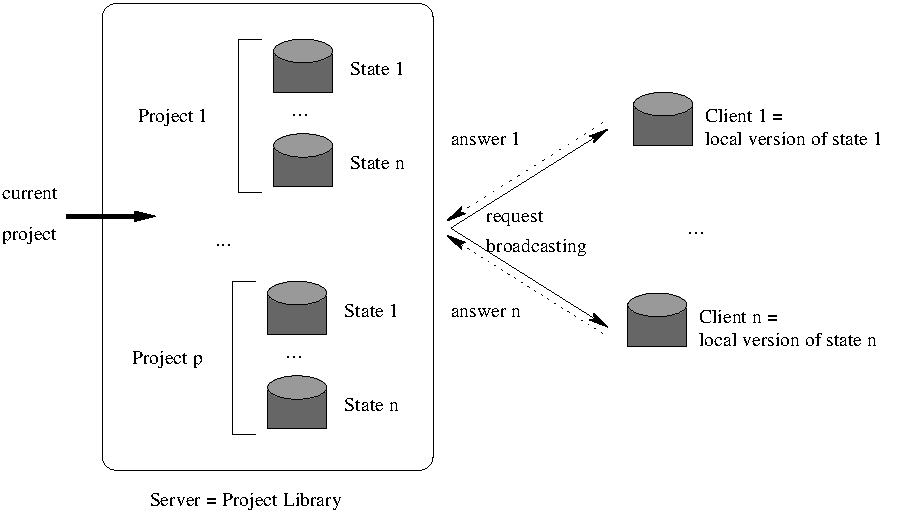
\includegraphics[viewport=0 0 440 246,width=0.99\textwidth]{mecanism.pdf}
    \caption{Interaction between the project library and your registered global
      data.}\label{fig:proj-mechanism}
  \end{figure}

\item It is part of the information saved on disk\index{Saving} for restoration
  in a later session\index{Loading}.
\item It may be part of a \emph{selection}\index{Selection} which is a
  consistent set of states\index{State!Selection|see{Selection}}.
  With such a selection,
  you can control on which states project operations are consistently applied
  (see Section~\ref{proj:selection}). For example, it is possible to clear all
  the states which depend on value analysis results.
\item It is possible to ensure inter-analysis consistency\index{Consistency} by
  setting state dependencies\index{State!Dependency}. For example, if the entry
  point\index{Entry Point} of the analyzed program is changed (using
  \texttt{Globals.set\_entry\_point}\scodeidx{Globals}{set\_entry\_point}), all
  the results of analyses depending on it (like value analysis' results) are
  automatically reset. If such a reset were not performed, the results of the
  value analysis would not be consistent anymore with the current entry point,
  leading to incorrect results.
\begin{example}
\scodeidx{Analysis}{is\_computed}
\sscodeidx{Eva}{Analysis}{is\_computed}
\scodeidx{Analysis}{compute}
\sscodeidx{Eva}{Analysis}{compute}
~

\begin{ocamlcode}
Eva.Analysis.compute();
Kernel.feedback "%B" (Eva.Analysis.is_computed ()); (* true *)
Globals.set_entry_point "f" true;
Kernel.feedback "%B" (Eva.Analysis.is_computed ()); (* false *)
\end{ocamlcode}
As the value analysis has been automatically reset when setting the entry point,
the above code outputs
\begin{logs}
[kernel] true
[kernel] false
\end{logs}
\end{example}
\end{itemize}

\subsubsection{State Registration: Overview}
\index{State!Registration|bfit}

For registering a new state, functor
\texttt{State\_builder.Register}\scodeidx{State\_builder}{Register} is
provided. Its use is described in Section~\ref{proj:lowlevel} but it is a
low-level functor which is usually difficult to apply in a correct
way. Higher-level functors are provided to the developer in modules
\texttt{State\_builder}\codeidx{State\_builder} and
\texttt{Cil\_state\_builder}\codeidx{Cil\_state\_builder} that allow the
developer to register states in a simpler way. They internally apply the
low-level functor in the proper way. Module \texttt{State\_builder} provides
state builders for standard \caml datastructures like
hashtables\index{Hashtable} whereas \texttt{Cil\_state\_builder} does the same
for standard \cil datastructures (like hashtables indexed by AST
statements)\footnote{These datastructures are only mutable datastructures (like
  hashtables, arrays and references) because global states are always
  mutable.}. They are described in Section~\ref{proj:computation}.

\begin{important}
  Registering a new state must be performed when the plugin is
  initialized. Thus, using \caml \texttt{let module} construct to
  register the new state is forbidden (except if you really know what
  you are doing).
\end{important}

\subsection{Registering a New State}\label{proj:computation}
\index{State!Registration|bfit}

Here we explain how to register and use a state. Registration through the use of
the low-level functor \texttt{State\_builder.Register} is postponed in
Section~\ref{proj:lowlevel} because it is more tricky and rarely useful.

In most non-\framac applications, a state is a global mutable value. One can use
it to store results of analyses. For example, using this mechanism inside
\framac to create a \texttt{state} which would memoize\index{Memoization} some
information attached to statements would result in the following piece of code.
\codeidx{Kernel\_function}\sscodeidx{Datatype}{Ty}{t}
\scodeidx{Cil\_types}{varinfo}
\scodeidx{Cil\_datatype}{Stmt}\sscodeidx{Datatype}{S\_with\_collections}{Hashtbl}
\sscodeidx{Eva}{Analysis}{compute}
\begin{ocamlcode}
open Cil_datatype
type info = Kernel_function.t * Cil_types.varinfo
let state : info Stmt.Hashtbl.t = Stmt.Hashtbl.create 97
let compute_info (kf,vi) = ...
let memoize s =
  try Stmt.Hashtbl.find state s
  with Not_found -> Stmt.Hashtbl.add state s (compute_info s)
let run () = ... Eva.Analysis.compute (); ... memoize some_stmt ...
\end{ocamlcode}

However, if one puts this code inside \framac, it does not work because this
state is not registered as a \framac state. For instance, it is never saved on
the disk\index{Saving} and its value is never changed when setting the current
project to a new one. For this purpose, one has to transform the above code into
the following one. \scodeidx{Cil\_state\_builder}{Stmt\_hashtbl}
\scodeidx{Datatype}{Pair} \codeidx{Kernel\_function}
\scodeidx{Cil\_datatype}{Varinfo} \sscodeidx{Eva}{Analysis}{self}
\sscodeidx{Eva}{Analysis}{compute} \codeidx{memo}
\begin{ocamlcode}
module State =
  Cil_state_builder.Stmt_hashtbl
    (Datatype.Pair(Kernel_function)(Cil_datatype.Varinfo))
    (struct
      let size = 97
      let name = "state"
      let dependencies = [ Eva.Analysis.self ]
     end)
let compute_info (kf,vi) = ...
let memoize = State.memo compute_info
let run () = ... Eva.Analysis.compute (); ... memoize some_stmt ...
\end{ocamlcode}
A quick look on this code shows that the declaration of the state itself is more
complicated (it uses a functor application) but its use is
simpler. Actually what has changed?
\begin{enumerate}
\item To declare a new internal state, apply one of the predefined functors in
  modules \texttt{State\_builder}\codeidx{State\_builder} or
  \texttt{Cil\_state\_builder}\codeidx{Cil\_state\_builder} (see interfaces of
  these modules for the list of available modules). Here we use
  \texttt{Cil\_state\_builder.Stmt\_hashtbl} which provides a hashtable indexed
  by statements. The type of values associated to statements is a pair of
  \texttt{Kernel\_function.t} and
  \texttt{Cil\_types.varinfo}\scodeidx{Cil\_types}{varinfo}. The first argument
  of the functor is then the datatype\index{Datatype} corresponding to this type
  (see Section~\ref{type:datatype}). The second argument provides some
  additional information: the initial size of the hashtable\index{Hashtable} (an
  integer similar to the argument of \texttt{Hashtbl.create}), an unique
  name\index{State!Name} for the resulting state and its
  dependencies\index{State!Dependency|bfit}. This list of dependencies is built
  upon values \texttt{self}\codeidxdef{self} which are called \emph{state
    kind}\index{State!Kind|see{Kind}} (or simply \emph{kind}\index{Kind|bfit})
  and are part of any state's module (part of the signature of the low-level
  functor \texttt{State\_builder.Register}%
  \scodeidx{State\_builder}{Register}). This value represents the state itself
  as first-class value (like type values for \caml types, see
  Section~\ref{type:type-value}).
\item From outside, a state actually hides its internal representation in order
  to ensure some invariants: operations on states implementing hashtables do
  not take hashtables as arguments because they implicitly use the hidden
  hashtable. In our example, a predefined memo function is used in order to
  memoize\index{Memoization} the computation of \texttt{compute\_info}. This
  memoization function implicitly operates on the hashtable hidden in the
  internal representation of \texttt{State}.
\end{enumerate}

%\todo{Computation.apply\_once (?)}

\paragraph{Postponed dependencies}\index{State!Dependency!Postponed|bfit}

Sometimes, you want to access a state kind before defining it. That is
usually the case when you have two mutually-dependent states: the dependencies
of the first one provided when registering it must contain the state kind of
the second one which is created by registering it. But this second registration
also requires a list of dependencies containing the first state kind.

For solving this issue, it is possible to postpone the addition of a
state kind to dependencies until all modules have been initialized. However,
dependencies must be correct before anything serious is computed by \framac. So
the right way to do this is the use of the function
\texttt{Cmdline.run\_after\_extended\_stage}%
\scodeidx{Cmdline}{run\_after\_extended\_stage} (see
Section~\ref{adv:init} for advanced explanation about the way \framac is
initialized).
\begin{example}
Plug-in \texttt{from}\index{From} creates a \texttt{State}\index{State} exposed
via its API.

\noindent
\listingname{src/plugins/from/functionwise.ml}
\scodeidx{Kernel\_function}{Make\_Table}
\sscodeidx{Eva}{Analysis}{self}
\begin{ocamlcode}
module Tbl =
  Kernel_function.Make_Table
    (Function_Froms)
    (struct
       let name = "functionwise_from"
       let size = 97
       let dependencies = [ Eva.Analysis.self ]
     end)
let self = Tbl.self
\end{ocamlcode}
\listingname{src/plugins/from/from.ml}
\begin{ocamlcode}
let self = Functionwise.self
\end{ocamlcode}

Plug-in \texttt{pdg}\index{Plug-in!Pdg|see{Pdg}}\index{Pdg} uses
\texttt{from}\index{From} for computing its own internal state. So it declares
this dependency as follows.

\noindent\listingname{src/plugins/pdg/pdg\_tbl.ml}
\scodeidx{Kernel\_function}{Make\_Table}
\begin{ocamlcode}
module Tbl =
  Kernel_function.Make_Table
    (PdgTypes.Pdg)
    (struct
       let name = "Pdg.State"
       let dependencies = [] (* postponed because From.self may not exist yet *)
       let size = 97
    end)
let self = Tbl.self
\end{ocamlcode}
\listingname{src/plugins/pdg/register.ml}
\scodeidx{State\_dependency\_graph}{S.add\_codependencies}
\scodeidx{Cmdline}{run\_after\_extended\_stage}
\begin{ocamlcode}
let () =
  Cmdline.run_after_extended_stage
    (fun () ->
       State_dependency_graph.add_codependencies
         ~onto:Pdg_tbl.self
         [ From.self ])
\end{ocamlcode}
\end{example}

\paragraph{Dependencies over the AST}

Most internal states depend directly or indirectly on the AST of the current
project. However, the AST plays a special role as a state. Namely, it can be
changed in place, bypassing the project mechanism. In particular, it is possible
to add globals. Plugins that perform such changes should inform the kernel
when they are done using
\texttt{Ast.mark\_as\_changed}\scodeidxdef{Ast}{mark\_as\_changed} or
\texttt{Ast.mark\_as\_grown}\scodeidxdef{Ast}{mark\_as\_grown}. The latter
must be used when the only changes are additions, leaving existing nodes
untouched, while the former must be used for more intrusive changes.
In addition, it is possible to tell the kernel that a state is ``monotonic''
with respect to AST changes, in the sense that it does not need to be cleared
when nodes are added (the information that should be associated to the new
nodes will be computed as needed). This is done with the function
\texttt{Ast.add\_monotonic\_state}\scodeidxdef{Ast}{add\_monotonic\_state}.
\texttt{Ast.mark\_as\_grown} will not touch such a state, while
\texttt{Ast.mark\_as\_changed} will clear it.

\subsection{Direct Use of Low-level Functor \texttt{State\_builder.Register}}
\label{proj:lowlevel}

Functor \texttt{State\_builder.Register}%
\scodeidxdef{State\_builder}{Register} is the only functor which really
registers a state. All the others internally use it. In some cases (\eg if you
define your own mutable record used as a state), you have to use it. Actually,
in the \framac kernel\index{Kernel}, there are only three direct uses of this
functor over thousands of state registrations: so you will certainly never use
it.

This functor takes three arguments. The first and the third ones respectively
correspond to the datatype\index{Datatype} and to information (name and
dependencies) of the states\index{State!Name}%
\index{State!Dependency}: they are similar to the corresponding
arguments of the high-level functors (see Section~\ref{proj:computation}).

The second argument explains how to handle the \emph{local
  version}\index{State!Local Version|bfit} of the state under
registration. Indeed here is the key point: from the outside, only this local
version is used for efficiency purposes (remember
Figure~\ref{fig:proj-mechanism}). It would work even if projects do not
exist. Each project knows a \emph{global version}\index{State!Global
  Version|bfit}. The project management system \emph{automatically}
switches\index{Context Switch} the local version when the current
project\index{Project!Current} changes in order to conserve a physical
equality\index{Equality!Physical} between local version and current global
version. So, for this purpose, the second argument provides a type \texttt{t}
(type of values of the state) and five functions \texttt{create} (creation of a
new fresh state), \texttt{clear} (cleaning a state), \texttt{get} (getting a
state), \texttt{set} (setting a state) and \texttt{clear\_some\_projects} (how
to clear each value of type \texttt{project} in the state if any).

\begin{important}
The following invariants must
hold\index{Equality!Physical}\index{Equality!Structural}:\footnotemark
\begin{gather}
\texttt{create ()} \mbox{ returns a fresh value} \label{eq:create}\\
\forall \texttt{p} \mbox{ of type } \texttt{t},\,
\texttt{create () = (clear p; set p; get ())}\label{eq:clear}\\
\forall \texttt{p} \mbox{ of type } \texttt{t},\, \texttt{copy p} \mbox{
  returns a fresh value}
\label{eq:copy}\\
\forall \texttt{p1},\texttt{p2} \mbox{ of type } \texttt{t}
\mbox{ such that } \texttt{p1 != p2},\, \texttt{(set p1; get ()) != p2}
\label{eq:independance}
\end{gather}
\end{important}
\footnotetext{As usual in \caml, \texttt{=} stands for \emph{structural}
  equality while \texttt{==} (resp. \texttt{!=}) stands for \emph{physical}
  equality (resp. disequality).}

Invariant~\ref{eq:create} ensures that there is no sharing%
\index{State!Sharing} with any value of a same state: so each new project has
got its own fresh state. Invariant~\ref{eq:clear} ensures that cleaning
a state\index{State!Cleaning} resets it to its initial
value. Invariant~\ref{eq:copy} ensures that there is no sharing with any
copy. Invariant~\ref{eq:independance} is a local independence criterion which
ensures that modifying a local version does not affect any other version
(different from the global current one) by side effects\index{Side-Effect}.
\begin{example}
  To illustrate this, we show how functor
  \texttt{State\_builder.Ref}\scodeidx{State\_builder}{Ref} (registering a state
  corresponding to a reference) is implemented.
\scodeidx{Datatype}{S}
\begin{ocamlcode}
module Ref
  (Data: Datatype.S)
  (Info: sig include Info val default: unit -> Data.t end) =
struct
  type data = Data.t
  let create () = ref Info.default
  let state = ref (create ())
\end{ocamlcode}
Here we use an additional reference: our local version%
\index{State!Local Version} is a reference on the right value. We can
use it in order to safely and easily implement \texttt{get} and \texttt{set}
required by the registration.
\scodeidx{State\_builder}{Register}
\scodeidx{Datatype}{Ref}
\begin{ocamlcode}
  include Register
    (Datatype.Ref(Data))
    (struct
      type t = data ref (* we register a reference on the given type *)
      let create = create
      let clear tbl = tbl := Info.default
      let get () = !state
      let set x = state := x
      let clear_some_projects f x =
        if Data.mem_project f !x then begin clear x; true end else false
    end)
   (Info)
\end{ocamlcode}
For users of this module, we export ``standard'' operations which hide the
local indirection required by the project management system.
\begin{ocamlcode}
  let set v = !state := v
  let get () = !(!state)
  let clear () = !state := Info.default
end
\end{ocamlcode}
As you can see, the above implementation is error prone; in particular it uses
a double indirection (reference of reference). So be happy that higher-level
functors like \texttt{State\_builder.Ref} are provided which hide such
implementations from you.
\end{example}

\subsection{Using Projects}\label{proj:use}\index{Project!Use|bfit}

As said before, all operations are done by default on the current
project\index{Project!Current}. But sometimes plug-in developers have to
explicitly use another project, for example when the AST is
modified\index{AST!Modification} (usually through the use of a copy
visitor\index{Visitor!Copy}, see Section~\ref{adv:visitors}) or replaced (\eg if
a new one is loaded\index{Loading} from disk).

\begin{important}
  An AST must never be modified inside a
  project\index{AST!Modification}. If such an operation is required, you
  must either create a new project with a new AST, usually by using
  \texttt{File.init\_project\_from\_cil\_file}%
  \scodeidxdef{File}{init\_project\_from\_cil\_file}
  or \texttt{File.init\_project\_from\_visitor}%
  \scodeidxdef{File}{init\_project\_from\_visitor};
  or write the following line of code (see Section~\ref{proj:selection}):
  \scodeidx{Project}{clear}
  \scodeidx{State\_selection}{only\_dependencies}
  \scodeidx{Ast}{self}
  \begin{alltt}
  let selection = State_selection.only_dependencies Ast.self in
  Project.clear ~selection ()
  \end{alltt}
\end{important}

Operations over projects are grouped together in module
\texttt{Project}\codeidxdef{Project}. A project has type
\texttt{Project.t}\scodeidxdef{Project\_skeleton}{t}. Function
\texttt{Project.set\_current}\scodeidxdef{Project}{set\_current} sets the
current project on which all operations are implicitly performed.

\begin{example}\label{ex:set_current}
  Suppose that you saved\index{Saving} the current project into file
  \texttt{foo.sav} in a previous \framac session\index{Session|bfit}\footnote{A
    \emph{session} is one execution of \framac (through \texttt{frama-c} or
    \texttt{frama-c-gui}).} thanks to the following
  instruction.\scodeidx{Project}{save}
\begin{ocamlcode}
Project.save "foo.sav"
\end{ocamlcode}
In a new \framac session, executing the following lines of code (assuming the
value analysis has never been computed previously)
\sscodeidx{Eva}{Analysis}{is\_computed}
\scodeidx{Project}{current}
\scodeidx{Project}{load}
\scodeidx{Project}{set\_current}
\sscodeidx{Eva}{Analysis}{compute}
\scodeidx{Project}{IOError}
\begin{ocamlcode}
let print_computed () =
  Kernel.feedback "%B" (Eva.Analysis.is_computed ())
in
print_computed ();   (* false *)
let old = Project.current () in
try
  let foo = Project.load ~name:"foo" "foo.sav" in
  Project.set_current foo;
  Eva.Analysis.compute ();
  print_computed ();   (* true *)
  Project.set_current old;
  print_computed ()    (* false *)
with Project.IOError _ ->
  Kernel.abort "error while loading"
\end{ocamlcode}
displays
\begin{logs}
[kernel] false
[kernel] true
[kernel] false
\end{logs}
This example shows that the value analysis has been computed only in project
\texttt{foo} and not in project \texttt{old}.
\end{example}

\begin{important}
An important invariant of \framac is: if $p$ is the current project before
running an analysis, then $p$ will be the current project after running it. It
is the responsibility of any plug-in developer to enforce this invariant for
his/her own analysis.
\end{important}

To be sure to enforce the above-mentioned invariant, the project library
provides an alternative to the use of
\texttt{Project.set\_current}\scodeidx{Project}{set\_current}:
\texttt{Project.on}\scodeidxdef{Project}{on} applies an operation on a
given project without changing the current project (\emph{i.e.} locally switch
the current project in order to apply the given operation and, afterwards,
restore the initial context)\index{Context Switch}.
\begin{example}
The following code is equivalent to the one given in
Example~\ref{ex:set_current}.
\begin{ocamlcode}
let print_computed () =
  Value_parameters.feedback "%B" (Eva.Analysis.is_computed ())
in
print_computed ();   (* false *)
try
  let foo = Project.load ~name:"foo" "foo.sav" in
  Project.on foo
    (fun () -> Eva.Analysis.compute (); print_computed () (* true *)) ();
  print_computed ()    (* false *)
with Project.IOError _ ->
  exit 1
\end{ocamlcode}
It displays
\begin{logs}
false
true
false
\end{logs}
\end{example}

\subsection{Selections}\label{proj:selection}\index{Selection|bfit}

Most operations working on a single project (\eg
\texttt{Project.clear}\scodeidx{Project}{clear} or
\texttt{Project.on}\scodeidx{Project}{on}) have an optional parameter
\texttt{selection} of type
\texttt{State\_selection.t}\codeidx{State\_selection}. This parameter allows the
developer to specify on which states\index{State} the operation
applies. A \emph{selection} is a set of states which allows the developer to
consistently handle state dependencies\index{State!Dependency}.
\begin{example}
  The following statement clears all the results of the value analysis and all
  its dependencies in the current project.\index{State!Cleaning}
  \scodeidx{Project}{clear}
  \scodeidx{State\_selection}{with\_dependencies}
  \sscodeidx{Eva}{Analysis}{self}
\begin{ocamlcode}
let selection = State_selection.with_dependencies Eva.Analysis.self in
Project.clear ~selection ()
\end{ocamlcode}
The selection explicitly indicates that we also want to clear all the states
which depend on the value analysis' results\index{State!Dependency}.
\end{example}

\begin{important}
  Use selections carefully: if you apply a function $f$ on a selection $s$ and
  $f$ handles a state which does not belong to $s$, then the computed result by
  \framac is potentially incorrect\index{Consistency}.
\end{important}

\begin{example}
The following statement applies a function \texttt{f} in the project \texttt{p}
(which is not the current one). For efficiency purposes, we restrict the
considered states to the command line options (see Section~\ref{adv:cmdline}).
\scodeidx{Project}{on}
\scodeidxdef{Parameter\_state}{get\_selection}
\begin{ocamlcode}
Project.on ~selection:(Parameter_state.get_selection ()) p f ()
\end{ocamlcode}
This statement only works if \texttt{f} only handles values of the command line
options\index{Command Line!Option}. If it tries to get the value of another
state, the result is unspecified \emph{and all actions using any state of the
  current project\index{Project!Current} and of project \texttt{p} also become
  unspecified}.
\end{example}

%%%%%%%%%%%%%%%%%%%%%%%%%%%%%%%%%%%%%%%%%%%%%%%%%%%%%%%%%%%%%%%%%%%%%%%%%%%%%%%

\section{Command Line Options}\label{adv:cmdline}
\index{Command Line!Option|bfit}

\begin{prereq}
  Knowledge of the \caml module system.
\end{prereq}

Values associated with command line options are called
\emph{parameters}\index{Parameters|bfit}. The parameters of the \framac kernel
are stored in module \texttt{Kernel}\codeidxdef{Kernel} while the
plug-in specific ones have to be defined in the plug-in source
code.

\subsection{Definition}\label{options:definition}

In \framac, a parameter is represented by a value of type
\texttt{Typed\_parameter.t}\codeidxdef{Typed\_parameter}
\sscodeidx{Datatype}{Ty}{t}
and by a module implementing the signature
\texttt{Parameter\_sig.S}\scodeidxdef{Parameter\_sig}{S}. The first
representation is a low-level one required by emitters\index{Emitter} (see
Section~\ref{adv:annotations}) and the GUI. The second one provides a high-level
API: each parameter is indeed a state\index{State} (see
Section~\ref{proj:states}).  Several signatures extending
\texttt{Parameter\_sig.S} are provided in order to deal with the usual parameter
types. For example, there are signatures
\texttt{Parameter\_sig.Int}\scodeidxdef{Parameter\_sig}{Int} and
\texttt{Parameter\_sig.Bool}\scodeidxdef{Parameter\_sig}{Bool} for integer and
boolean parameters. Mostly, these signatures provide getters and setters for
modifying parameter values.

Implementing such an interface is very easy thanks to a set of functors provided
by the output module of
\texttt{Plugin.Register}\scodeidx{Plugin}{Register}. Indeed, you have just to
choose the right functor according to your option type and potentially
the wished default value. Below are some examples of such functors
(see the signature
\texttt{Parameter\_sig.Builder}\scodeidx{Parameter\_sig}{Builder} for an
exhaustive list).
\begin{enumerate}
\item \texttt{False}\sscodeidxdef{Parameter\_sig}{Builder}{False}
  (resp. \texttt{True}\sscodeidxdef{Parameter\_sig}{Builder}{True}) builds a
  boolean option initialized to \texttt{false} (resp. \texttt{true}).
\item \texttt{Int}\sscodeidxdef{Parameter\_sig}{Builder}{Int}
  (resp. \texttt{Zero}\sscodeidxdef{Parameter\_sig}{Builder}{Zero}) builds an
  integer option initialized to a specified value (resp. to \texttt{0}).
\item \texttt{String}\sscodeidxdef{Parameter\_sig}{Builder}{String}
  (resp. \texttt{Empty\_string}
  \sscodeidxdef{Parameter\_sig}{Builder}{Empty\_string}) builds a string option
  initialized to a specified value (resp. to the empty string \texttt{""}).
\item \texttt{String\_set}\sscodeidxdef{Parameter\_sig}{Builder}{String\_set}
  builds an option taking a set of strings in argument (initialized to the empty
  set).
\item
  \texttt{Kernel\_function\_set}%
\sscodeidxdef{Parameter\_sig}{Builder}{Kernel\_function\_set} builds an option
taking a set of kernel functions in argument (initialized to the empty set).
\end{enumerate}
Each functor takes as argument (at least) the name of the command line option
corresponding to the parameter and a short description for this option.

\begin{example}
  The parameter corresponding to the option \texttt{-occurrence} of the plug-in
  \texttt{occurrence} is the module \texttt{Print} (defined in the file
  \texttt{src/plugins/occurrence/options.ml}). It is implemented as follows.
  \sscodeidx{Parameter\_sig}{Builder}{False}
\begin{ocamlcode}
module Print =
  False
    (struct
       let option_name = "-occurrence"
       let help = "print results of occurrence analysis"
     end)
\end{ocamlcode}
So it is a boolean parameter initialized by default to
\texttt{false}. The declared interface for this module is simply
\scodeidx{Parameter\_sig}{Bool}
\begin{ocamlcode}
module Print: Parameter_sig.Bool
\end{ocamlcode}

Another example is the parameter corresponding to the option
\texttt{-impact-pragma} of the plug-in \texttt{impact}. This parameter is
defined by the module \texttt{Pragma} (defined in the file
\texttt{src/plugins/impact/options.ml}). It is implemented as follows.
\sscodeidx{Parameter\_sig}{Builder}{Kernel\_function\_set}
\begin{ocamlcode}
module Pragma =
  Kernel_function_set
    (struct
       let option_name = "-impact-pragma"
       let arg_name = "f1, ..., fn"
       let help = "use the impact pragmas in the code of functions f1,...,fn"
     end)
\end{ocamlcode}
Thus it is a set of \texttt{kernel\_function}s initialized by default to
the empty set. \framac uses
the field \texttt{arg\_name} in order to print the name of the argument when
displaying help. The field \texttt{help} is the help message itself. The
Interface for this module is simple:
\scodeidx{Parameter\_sig}{Kernel\_function\_set}
\begin{ocamlcode}
module Pragma: Parameter_sig.Kernel_function_set
\end{ocamlcode}
\end{example}

\begin{convention}
Parameters of a same plug-in \texttt{plugin} should belong to a module called
\texttt{Options}, \texttt{Plugin\_options}, \texttt{Parameters} or
\texttt{Plugin\_parameters} inside the plug-in directory.
\end{convention}

Using a kernel parameters or a parameter of your own plug-in is very simple:
you have simply to call the function \texttt{get} corresponding to your
parameter.
\scodeidx{Kernel}{Unicode}
\begin{example}
To know whether \framac uses unicode, just write
\begin{ocamlcode}
Kernel.Unicode.get ()
\end{ocamlcode}

Inside the plug-in \texttt{From}, just write
\scodeidx{From\_parameters}{ForceCallDeps}
\begin{ocamlcode}
From_parameters.ForceCallDeps.get ()
\end{ocamlcode}
in order to know whether callsite-wise dependencies have been required.
\end{example}

Using a parameter of a plug-in $p$ in another plug-in $p'$ requires the use of
module \texttt{Dynamic.Parameter}\scodeidx{Dynamic}{Parameter}: since the
module defining the parameter is not visible from the outside of its plug-in,
you have to use the dynamic API of plug-in $p$ in which $p$'s parameters are
automatically registered (see Section~\ref{adv:dynamic-registration}). The
module \texttt{Dynamic.Parameter} defines sub-modules which provide easy access
to parameters according to their \caml types.
\sscodeidx{Dynamic}{Parameter}{Bool}
\begin{example}
Outside the plug-in \texttt{From}, just write
\begin{ocamlcode}
Dynamic.Parameter.Bool.get "-calldeps" ()
\end{ocamlcode}
in order to know whether callsite-wise dependencies have been required.
\end{example}

\subsection{Tuning}\label{options:tuning}

It is possible to modify the default behavior of command line options in several
ways by applying functions just before or just after applying the functor
defining the corresponding parameter.

Functions which can be applied afterwards are defined in the output signature of
the applied functor.
\begin{example}
Here is how the option "-slicing-level" restricts the range of its argument to
the interval $[0;3]$.
\begin{ocamlcode}
module Calls =
  Int
    (struct
       let option_name = "-slicing-level"
       let default = 2
       let arg_name = ""
       let help = "..." (* skipped here *)
       end)
let () = Calls.set_range ~min:0 ~max:3
\end{ocamlcode}
\end{example}

Functions which can be applied before applying the functor are defined in the
module \texttt{Parameter\_customize}\codeidxdef{Parameter\_customize}.
\begin{example}
Here is how the opposite of option "-safe-arrays" is renamed into
"-unsafe-arrays" (otherwise, by default, it would be "-no-safe-arrays").
\scodeidx{Parameter\_customize}{set\_negative\_option\_name}
\scodeidx{Kernel}{SafeArrays}
\begin{ocamlcode}
let () = Parameter_customize.set_negative_option_name "-unsafe-arrays"
module SafeArrays =
  True
    (struct
       let module_name = "SafeArrays"
       let option_name = "-safe-arrays"
       let help = "for arrays that are fields inside structs, assume that €
                   accesses are in bounds"
     end)
\end{ocamlcode}
\end{example}

%%%%%%%%%%%%%%%%%%%%%%%%%%%%%%%%%%%%%%%%%%%%%%%%%%%%%%%%%%%%%%%%%%%%%%%%%%%%%%%

\section{Initialization Steps}\label{adv:init}
\index{Initialization|bfit}
\index{Module Initialization|see{Initialization}}
\index{Plug-in!Initialization|see{Initialization}}

\begin{prereq}
  Knowledge of linking of \caml files.
\end{prereq}

\begin{important}
  In a standard way, \framac modules are initialized in the link
  order\index{Linking} which remains mostly unspecified, so you have to use
  side-effects\index{Side-Effect} at module initialization time carefully.
\end{important}

This section details the different stages of the \framac boot process
to help advanced plug-in developers interact more deeply with
the kernel process. It can also be useful for debugging initialization
problems.

As a general rule, plug-in routines must never be executed at link time. Any
useful code, be it for registration, configuration or \textsf{C}-code analysis,
should be registered as \emph{function hooks} to be executed at a proper time
during the \framac boot process. In general, registering and executing a hook is
tightly coupled with handling the command line parameters.

The parsing of the command line parameters is performed in several
\emph{phases} and \emph{stages}
\index{Command Line!Parsing},
each one dedicated to specific operations.
Following the general rule stated at the beginning of this section, even
the kernel services of \framac are internally registered as hooks routines to
be executed at a specific stage of the initialization process, among plug-ins
ones.

From the plug-in developer point of view, the hooks are registered by
calling the \texttt{run\_after\_$xxx$\_stage} routines in
\texttt{Cmdline}\codeidx{Cmdline} module and \texttt{extend} routine
in the \texttt{Boot.Main}\sscodeidx{Boot}{Main}{extend} module.

The initialization phases and stages of \framac are described below, in
their execution order.

\begin{enumerate}[A --]

\item \textbf{The Initialization Stage:}\index{Initialization} this stage
  initializes \framac compilation units, following some \emph{partially}
  specified order. More precisely:
  \begin{enumerate}[1.]
  \item the architecture dependencies depicted on
    Figure~\ref{fig:architecture} (cf.~p.~\pageref{archi:general}) are
    respected. In particular, the kernel services are linked first,
    \emph{then} the kernel integrated types for plug-ins, and
    \emph{finally} the plug-ins are linked in unspecified order;
  \item when the GUI\index{Plug-in!GUI} is present, for any plug-in
    $p$, the non-gui modules of $p$ are always linked \emph{before}
    the gui modules of $p$;
  \item finally, the module \texttt{Boot}\codeidxdef{Boot} is linked at the
    very end of this stage.
  \end{enumerate}

  Plug-in developers cannot customize this stage. In particular, the module
  \texttt{Cmdline}\codeidx{Cmdline} (one of the first linked modules, see
  Figure~\ref{fig:architecture}) performs a very early configuration stage,
  such as setting the global verbosity and debugging levels.

\item \label{stage:early} \textbf{The Early Stage:} this stage initializes the
  kernel services. More precisely:
  \begin{enumerate}[(a)]
  \item first, the parsing of command line options registered for the
    \texttt{Cmdline.Early}\sscodeidxdef{Cmdline}{stage}{Early} stage;
  \item then, all functions registered through
    \texttt{Cmdline.run\_after\_early\_stage}%
    \scodeidxdef{Cmdline}{run\_after\_early\_stage} are executed in an
    unspecified order.
  \end{enumerate}

\item \label{stage:extending} \textbf{The Extending Stage:}\index{Linking} the searching and
  loading of dynamically linked plug-ins, scripts and
  modules is performed at this stage. More precisely:

  \begin{enumerate}[(a)]
  \item the command line options registered for the
    \texttt{Cmdline.Extending}\sscodeidxdef{Cmdline}{stage}{Extending} stage
    are treated, such as \texttt{-load-module}

  \item the hooks registered through
    \texttt{Cmdline.run\_during\_extending\_stage}
    \scodeidxdef{Cmdline}{run\_during\_extending\_stage} are executed. Such
    hooks include kernel function calls for searching, loading and linking the
    various plug-ins and scripts compilation units, with respect to
    the command line options parsed during stages~\ref{stage:early}
    and~\ref{stage:extending}.
  \end{enumerate}

\item \textbf{The Running Phase:} the command line is split into several
  groups of command line arguments, each of them separated by an option
  \texttt{-then} or an option \texttt{-then-on $p$} (thus if there is $n$
  occurrences of \texttt{-then} or \texttt{-then-on $p$}, then there are $n+1$
  groups). For each group, the following stages are executed in sequence: all
  the stages are executed on the first group provided on the command line, then
  they are executed on the second group, and so on.

\begin{enumerate}[1.]

\item \textbf{The Extended Stage:} this step is reserved for commands which
  require that all plug-ins are loaded but which must be executed very
  early. More precisely:

  \begin{enumerate}[(a)]
  \item the command line options registered for the
    \texttt{Cmdline.Extended}\sscodeidxdef{Cmdline}{stage}{Extended} stage
    are treated, such as \texttt{-verbose-*} and \texttt{-debug-*};

  \item the hooks registered through
    \texttt{Cmdline.run\_after\_extended\_stage}%
    \scodeidxdef{Cmdline}{run\_after\_extended\_stage}.
    Most of these registered hooks come from postponed internal-state
    dependencies\index{State!Dependency!Postponed} (see
    Section~\ref{proj:computation}).
  \end{enumerate}

  Remark that both statically and dynamically linked plug-ins have
  been loaded at this stage. Verbosity and debug level for each
  plug-in are determined during this stage.

\item \textbf{The Exiting Stage:} this step is reserved for commands
  that make \framac exit before starting any analysis at all, such as
  printing help information:
  \begin{enumerate}[(a)]

  \item the command line options registered for the
    \texttt{Cmdline.Exiting}\sscodeidxdef{Cmdline}{stage}{Exiting} stage
    are treated;

  \item the hooks registered through
    \texttt{Cmdline.run\_after\_exiting\_stage}
    \scodeidxdef{Cmdline}{run\_after\_exiting\_stage} are executed in
    an unspecified order. All these functions should do nothing (using
    \texttt{Cmdline.nop}\scodeidxdef{Cmdline}{nop}) or raise
    \texttt{Cmdline.Exit}\scodeidxdef{Cmdline}{Exit} for stopping \framac
    quickly.

  \end{enumerate}

\item \textbf{The Loading Stage:} this is where the initial state of \framac
  can be replaced by another one. Typically, it would be loaded from disk
  through the \texttt{-load} option\index{Loading}. As
  for the other stages:
  \begin{enumerate}[(a)]

  \item first, the command line options registered for the
    \texttt{Cmdline.Loading}\sscodeidxdef{Cmdline}{stage}{Loading} stage
    are treated;

  \item then, the hooks registered through
    \texttt{Cmdline.run\_after\_loading\_stage}
    \scodeidxdef{Cmdline}{run\_after\_loading\_stage} are executed in
    an unspecified order. These functions actually change the initial
    state of \framac with the specified one. The \framac kernel
    verifies as far as possible that only one new-initial state has
    been specified.
  \end{enumerate}

  Normally, plug-ins should never register hooks for this stage unless they
  actually set a different initial state than the default one. In such a case:

  \begin{important}
    They must call the function
    \texttt{Cmdline.is\_going\_to\_load}
    \scodeidxdef{Cmdline}{is\_going\_to\_load} while initializing.
  \end{important}

\item \textbf{The Configuring Stage:} this is the usual place for
  plug-ins to perform special initialization routines if necessary,
  \emph{before} having their main entry points executed. As for
  previous stages:

  \begin{enumerate}[(a)]
  \item first, the command line options registered for the
    \texttt{Cmdline.Configuring}\sscodeidxdef{Cmdline}{stage}{Configuring} stage
    are treated. Command line parameters that do not begin by a hyphen
    (character \texttt{'-'}) are \emph{not} options and are treated as
    \textsf{C} files. Thus they are added to the list of files to be
    preprocessed or parsed for building the \texttt{AST} (on demand);
  \item then, the hooks registered through
    \texttt{Cmdline.run\_after\_configuring\_stage}
    \scodeidxdef{Cmdline}{run\_after\_configuring\_stage} are executed
    in an unspecified order.
  \end{enumerate}

\item \textbf{The Setting Files Stage:} this stage sets the \C files to analyze
  according to those indicated on the command line. More precisely:

  \begin{enumerate}[(a)]
  \item first, each argument of the command line which does not begin by a
    hyphen (character \texttt{'-'}) is registered for later analysis;
  \item then, the hooks registered through
    \texttt{Cmdline.run\_after\_setting\_files}
    \scodeidxdef{Cmdline}{run\_after\_setting\_files} are executed in an
    unspecified order.
  \end{enumerate}

\item \textbf{The Main Stage:} this is the step where plug-ins actually run
  their main entry points registered through
  \texttt{Boot.Main.extend}\sscodeidx{Boot}{Main}{extend}. For all intents and purposes, you should consider
  that this stage is the one where these hooks are executed.

\end{enumerate}

\end{enumerate}

%%%%%%%%%%%%%%%%%%%%%%%%%%%%%%%%%%%%%%%%%%%%%%%%%%%%%%%%%%%%%%%%%%%%%%%%%%%%%%%

\section{Customizing the AST creation}\label{sec:customizing-ast}
\begin{prereq}
  None.
\end{prereq}

Plug-ins may modify the way source files are transformed into the AST
over which the analyses are performed. Customization of the front-end of
\framac can be done at several stages.

\begin{enumerate}[A --]
\item\textbf{Parsing:} this stage takes care of converting an individual source
file into a parsed AST (a.k.a Cabs, which differs from the type-checked AST on
which most analyses operate). By default, source files are treated as C files,
possibly needing a preprocessing phase. It is possible to tell Frama-C to use
another parser for files ending with a given suffix by registering this
parser with the \texttt{File.new\_file\_type}\scodeidxdef{File}{new\_file\_type}
function. Suffixes \texttt{.h}, \texttt{.i}, \texttt{.c} and \texttt{.ci}
are reserved for
Frama-C kernel. The registered parser is supposed to return a pair consisting
of a type-checked AST (\verb+Cil_types.file+\scodeidx{Cil\_types}{file}) and
a parsed AST (\verb+Cabs.file+\scodeidx{Cabs}{file}). The former can be obtained
from the latter with the \verb+Cabs2cil.convFile+\scodeidx{Cabs2cil}{convFile}
function, which guarantees that the resulting \verb+Cil_types.file+ respects
all invariants expected by the Frama-C kernel.
\item\textbf{Type-checking:} a normal \verb+Cabs.file+ ({\it i.e.} not obtained
through a custom parsing function) can be transformed before being
type-checked. Transformation hooks are registered through
\verb+Frontc.add_syntactic_transformation+%
\scodeidxdef{Frontc}{add\_syntactic\_transformation}.
\item\textbf{After linking:} Once all source files have been processed, they
  are all linked together in a single AST. Transformations can be performed
  on the resulting AST at two stages:
  \begin{enumerate}[1.]
  \item before clean-up ({\it i.e.} removal of useless temporary variables
    and prototypes that are never called). At that stage, global tables indexing
    information related to the AST have not yet been filled.
  \item after clean-up. At this stage, index tables are filled, and can thus
    be used. On the other hand, the transformation must take care itself
    of keeping in sync the AST and the tables
  \end{enumerate}
  Registering a transformation for this stage is done through the function
  \verb+File.add_code_transformation_before_cleanup+%
  \scodeidxdefsmall{File}{add\_code\_transformation\_before\_cleanup}
  (respectively \verb+File.add_code_transformation_after_cleanup+%
  \scodeidxdefsmall{File}{add\_code\_transformation\_after\_cleanup}). If such a
  transformation modify the control-flow graph of a function \texttt{f}, in
  particular by adding statements, it must call
  \verb|File.must_recompute_cfg|\scodeidxdef{File}{must\_recompute\_cfg}, in
  order to have the graph recomputed afterwards.
\end{enumerate}

%%%%%%%%%%%%%%%%%%%%%%%%%%%%%%%%%%%%%%%%%%%%%%%%%%%%%%%%%%%%%%%%%%%%%%%%%%%%%%%

\section{Customizing the machine model}\label{sec:customizing-machdep}
\index{Machine model}

\begin{prereq}
  None.
\end{prereq}

\subsection{Generating a custom model}\label{sec:gener-cust-model}
Several aspects of the C standard that are implementation-defined, such as
the width of standard integer types, endianness, signedness of the
\texttt{char} type, etc., as well as a few compiler and architecture specific
features, can be customized using a \texttt{machdep} configuration,
defining a new machine model.

Machine models are described as \texttt{YAML} files, following the
\texttt{machdeps/machdep-schema.yaml} schema in frama-c installed files.
Predefined machdeps are also located in the \texttt{machdeps} directory
of \framac's \texttt{SHARE} directory and can be used as reference for
defining new \texttt{machdep}s by hand. It is also possible to automatically
generate an \texttt{YAML} file with the \texttt{make\_machdep.py} script in
the \texttt{machdeps/make\_machdep} directory. This script requires a
C11-compliant cross-compiler for the architecture you want to describe.
Its main options are:
\begin{description}
\item \texttt{-compiler <c>}: the cross-compiler to be used for generating
  the machdep.
\item \texttt{-cpp-arch-flags <flag>}: an option given to the compiler for
selecting the desired architecture. Multiple occurrences of this option can
occur if you want to pass several options.
\item \texttt{-o <file>}: put the generated YAML into the given file (default
is to use standard output).
\item \texttt{--help}: outputs the list of all options of the script.
\end{description}

Note that for some compiler setups, notably for non-POSIX compilation targets,
the script may fail to find an appropriate value for some fields and will
instead put some default value. In that case, warnings will give the names of
the problematic fields. Since the issue likely stems from the fact that the
corresponding C feature is not supported on the compilation target in the first
place, in practice, such feature is not expected to be found in code written for
such target. However, users are invited to review the generated YAML and
provide more appropriate values for these fields if needed.

In order to communicate machine-related information to the preprocessor (notably
the value of standard macros), \framac generates a specific header,
\verb+__fc_machdep.h+, that is automatically included by the standard headers from
\framac's standard C library. Field \verb+custom_defs+ of the YAML file allows
customizing this header (see next section for more information).

\subsection{Machdep record fields}\label{sec:machdep-fields}

Each field of the machdep is succintly described in the
\verb+machdep-schema.yaml+ file.
We present below a thorough description of each field.

\paragraph{Meta-data}
\begin{description}
\item[\texttt{version}]: human-readable textual description of the machdep.
\item[\texttt{machdep\_name}]: name of the machdep, must only contain alphanumeric
  characters or underscore (\verb+_+). If it is e.g. \verb+custom_name+, the generated header will
  define a macro of the form \verb+__FC_MACHDEP_CUSTOM_NAME+.
\item[\texttt{compiler}]: defines whether special compiler-specific extensions
  will be enabled. It should be one of the strings below:
  \begin{itemize}
  \item[\texttt{msvc}]: enables \verb+Cil.msvcMode+, that is,
    MSVC (Visual Studio)-specific extensions;
  \item[\texttt{gcc}]: enables \verb+Cil.gccMode+, that is,
    GCC-specific extensions;
  \item[\texttt{generic}] (or any other string): no special
    compiler-specific extensions.
  \end{itemize}
  Note that some compiler extensions, such as attributes, are always enabled.
\item[\texttt{cpp\_arch\_flags}]: list of arguments used by the compiler to
  select the corresponding architecture, e.g. \verb+["-m32"]+ for a 32-bit
  machdep. Older versions (up to 26.x - Iron) of \framac did pass these flags to the preprocessor,
  in order for it to define a set of built-in macros related to said architecture.
  Current versions do not use this field, and rely on \texttt{\texttt{custom\_defs}}
  containing the appropriate definitions.
  Note that, in practice, very few programs rely on such predefined macros,
  such as \verb+__x86_64+ and \verb+__i386+.
\end{description}
\paragraph{Standard sizes and alignment constraints}
\begin{description}
  \item[\texttt{sizeof\_short}]: size (in bytes) of the \verb+short+ type.
  \item[\texttt{sizeof\_int}]: size (in bytes) of the \verb+int+ type.
  \item[\texttt{sizeof\_long}]: size (in bytes) of the \verb+long+ type.
  \item[\texttt{sizeof\_longlong}]: size (in bytes) of the \verb+long long+
    type.
    Note that machdeps (for compiler \verb+"gcc"+ in particular) must always
    have at least one type that is 8 bytes wide, which is typically
    \verb+long long+.
  \item[\texttt{sizeof\_ptr}]: size (in bytes) of an object (non-function)
    pointer.
  \item[\texttt{sizeof\_float}]: size (in bytes) of a single-precision floating
    point. In implementations compliant with ISO/IEC/IEEE 60559 - IEEE 754,
    this is always 4.
  \item[\texttt{sizeof\_double}]: size (in bytes) of a double-precision floating
    point. In implementations compliant with ISO/IEC/IEEE 60559 - IEEE 754,
    this is always 8.
  \item[\texttt{sizeof\_longdouble}]: size (in bytes) of a \verb+long double+
    floating point.
    Note: type \verb+long double+ is currently not supported by existing
    \framac plugins,  but this field exists for future expansion, and
    to compute \verb+sizeof+ of aggregates properly.
  \item[\texttt{sizeof\_void}]: the result of evaluating \verb+sizeof(void)+
    by the compiler (or negative if unsupported).
  \item[\texttt{sizeof\_fun}]: the result of evaluating \verb+sizeof(f)+, where
    \verb+f+ is a function ({\em not} a function pointer) by the compiler
    (or negative if unsupported).
  \item[\texttt{alignof\_short}]: the result of evaluating
    \verb+_Alignof(short)+.
  \item[\texttt{alignof\_int}]: the result of evaluating \verb+_Alignof(int)+.
  \item[\texttt{alignof\_long}]: the result of evaluating \verb+_Alignof(long)+.
  \item[\texttt{alignof\_longlong}]: the result of evaluating
    \verb+_Alignof(long long)+.
  \item[\texttt{alignof\_ptr}]: the result of evaluating \verb+_Alignof(char*)+
    (or any other pointer, including function pointers).
  \item[\texttt{alignof\_float}]: the result of evaluating
    \verb+_Alignof(float)+.
  \item[\texttt{alignof\_double}]: the result of evaluating
    \verb+_Alignof(double)+.
  \item[\texttt{alignof\_longdouble}]: the result of evaluating
    \verb+_Alignof(long double)+.
  \item[\texttt{alignof\_str}]: the result of evaluating \verb+_Alignof("a")+
    (a literal string).
  \item[\texttt{alignof\_fun}]: the result of evaluating \verb+_Alignof(f)+,
    where \verb+f+ is a function (or negative if unsupported).
  \item[\texttt{alignof\_aligned}]: the default alignment of a type having the
    \verb+aligned+ attribute (or 1 if unsupported). This corresponds to the
    default alignment when using \verb+#pragma packed()+ without a numeric
    argument.
\end{description}

\paragraph{Standard types}

\begin{description}
\item[\texttt{int\_fast8\_t}]: a string containing the actual type that
  \verb+int_fast8_t+ expands to. Usually \verb+signed char+.
\item[\texttt{int\_fast16\_t}]: a string containing the actual type that
  \verb+int_fast16_t+ expands to. Usually \verb+int+ or \verb+long+.
\item[\texttt{int\_fast32\_t}]: a string containing the actual type that
  \verb+int_fast_32_t+ expands to. Usually \verb+int+ or \verb+long+.
\item[\texttt{int\_fast64\_t}]: a string containing the actual type that
  \verb+int_fast64_t+ expands to. Usually \verb+long+ or \verb+long long+.
\item[\texttt{uint\_fast8\_t}]: a string containing the actual type that
  \verb+uint_fast8_t+ expands to. Usually \verb+unsigned char+.
\item[\texttt{uint\_fast16\_t}]: a string containing the actual type that
  \verb+uint_fast16_t+ expands to. Usually \verb+unsigned int+ or \verb+unsigned long+.
\item[\texttt{uint\_fast32\_t}]: a string containing the actual type that
  \verb+uint_fast_32_t+ expands to. Usually \verb+unsigned int+ or \verb+unsigned long+.
\item[\texttt{uint\_fast64\_t}]: a string containing the actual type that
  \verb+uint_fast64_t+ expands to. Usually \verb+unsigned long+ or
  \verb+unsigned long long+.
\item[\texttt{intptr\_t}]: a string containing the actual type that
  \verb+intptr_t+ expands to, e.g. \verb+long+
\item[\texttt{uintptr\_t}]: a string containing the actual type that
  \verb+uintptr_t+ expands to, e.g. \verb+unsigned long+
\item[\texttt{size\_t}]: a string containing the actual type that
  \verb+size_t+ expands to, e.g. \verb+unsigned long+.
\item[\texttt{ssize\_t}]: a string containing the actual type that
  \verb+ssize_t+ expands to, e.g. \verb+long+
\item[\texttt{wchar\_t}]: a string containing the actual type that
  \verb+wchar_t+ expands to. If unsupported, you can use \verb+int+.
\item[\texttt{ptrdiff\_t}]: a string containing the actual type that
  \verb+ptrdiff_t+ expands to. If unsupported, you can use \verb+int+.
\item[\texttt{sig\_atomic\_t}]: a string containing the actual type that
  \verb+sig_atomic_t+ expands to (i.e. an integer type that can be
  accessed atomically even in presence of interrupts).
\item[\texttt{time\_t}]: a string containing the actual type that
  \verb+time_t+ expands to (i.e. an integer type that can hold time
  values in seconds).
\item[\texttt{wint\_t}]: a string containing the actual type that
  \verb+wint_t+ expands to (i.e. an integer type capable of holding any
  \verb+wchar_t+ and \verb+WEOF+)
\end{description}

\paragraph{Standard macros}

Note that all fields described in this paragraph have \texttt{string} values,
even if they denote numeric constants. In order to avoid errors when loading the
YAML file, you can force them to be considered as strings by enclosing them between
single or double quotes, as in \verb+eof: '(-1)'+ (as a sidenote, negative values
should be enclosed in parentheses, in order to ensure safe macro expansions).

\begin{description}
  \item[\texttt{bufsiz}]: value of the \texttt{BUFSIZ} macro, i.e. the size
    of buffers used by I/O functions in \texttt{stdio.h}.
  \item[\texttt{eof}]: value of the \texttt{EOF} macro, the value returned by input
    functions in \texttt{stdio.h} to indicate the end of the stream.
  \item[\texttt{errno}]: list of possible errors with their numeric value. In order
    to be easier to read, the content of this field is in fact written itself as an
    object whose fields are the name of the errors. For instance, for a machdep defining
    only the three errors mandated by the C standard, we would have:
    \begin{verbatim}
    errno:
        edom: 1
        eilseq: 2
        erange: 3
    \end{verbatim}
  \item[\texttt{filename\_max}]: value of the \texttt{FILENAME\_MAX} macro, which
    denotes the longest name that is guaranteed to be accepted by \texttt{fopen}.
  \item[\texttt{fopen\_max}]: value of the \texttt{FOPEN\_MAX} macro, which denotes the
    greatest number of streams that can be simultaneously opened by the program.
  \item[\texttt{host\_name\_max}]: value of the \texttt{HOST\_NAME\_MAX} macro, which
    denotes the maximum length of a hostname (without terminating null byte).
  \item[\texttt{l\_tmpnam}]: value of the \texttt{L\_tmpnam} macro, which denotes
    the maximum size of a temporary filename as returned by \texttt{tmpnam}.
  \item[\texttt{mb\_cur\_max}]: value of the \texttt{MB\_CUR\_MAX} macro, which denotes
    the maximum number of bytes for a character in the current locale (usually
    \texttt{'1'}).
  \item[\texttt{nsig}]: number of possible signals (non-standard macro, can be left
    empty if undefined for the current machdep).
  \item[\texttt{path\_max}]: value of the \texttt{PATH\_MAX} macro, which denotes
    the maximum size (including terminating null) that can be stored in a buffer
    when returning a pathname.
  \item[\texttt{posix\_version}]: value of the \texttt{\_POSIX\_VERSION} macro.
    Leave empty on non-POSIX machdeps.
  \item[\texttt{rand\_max}]: value of the \texttt{RAND\_MAX} macro, which denotes
    the maximum value returned by \texttt{rand}.
  \item[\texttt{tmp\_max}]: value of the \texttt{TMP\_MAX} macro, which denotes
    the minimum number of temporary filenames returned by \texttt{tmpnam} that
    are guaranteed to be distinct.
  \item[\texttt{tty\_name\_max}]: value of the \texttt{TTY\_NAME\_MAX} macro, which
    denotes the maximum length of a terminal device name (including terminating null byte).
  \item[\texttt{weof}]: value of the \texttt{WEOF} macro, similar to \texttt{EOF},
    but for wide chars.
  \item[\texttt{wordsize}]: value of the \texttt{\_\_WORDSIZE} macro, which denotes
    the length of a word on the current architecture.
\end{description}

\paragraph{Other features}
\begin{description}
  \item[\texttt{char\_is\_unsigned}]: whether type \verb+char+ is unsigned.
  \item[\texttt{little\_endian}]: whether the machine is little endian or big
    endian\footnote{More exotic endianness such as mixed-endian are currently unsupported.}.
  \item[\texttt{has\_\_builtin\_va\_list}]: whether \verb+__builtin_va_list+
    is a (built-in) type known by the preprocessor.
  \item[\texttt{\_\_thread\_is\_keyword}]: whether \verb+__thread+ is a
    keyword (otherwise, it can be used as a standard identifier).
  \item[\texttt{custom\_defs}]: arbitrary text that will be appended
    verbatim at the
    end of the generated header file (this is empty in machdeps that are
    generated by the \texttt{make\_machdep.py} script).
\end{description}

%%%%%%%%%%%%%%%%%%%%%%%%%%%%%%%%%%%%%%%%%%%%%%%%%%%%%%%%%%%%%%%%%%%%%%%%%%%%%%%

\section{Visitors}\label{adv:visitors}\index{Visitor|bfit}

\begin{prereq}
  Knowledge of \caml object programming.
\end{prereq}

Module \texttt{Cil}\codeidx{Cil} offers a visitor\index{Visitor!Cil|bfit},
\verb+Cil.cilVisitor+\scodeidxdef{Cil}{cilVisitor},
that allows to traverse (parts of) an
AST\index{AST}. It is a class with one method per type of the AST, whose
default behavior is simply to call the method corresponding to its
children. This is a convenient way to perform local transformations over a
whole \verb+Cil_types.file+\scodeidx{Cil\_types}{file} by inheriting from it
and redefining a few methods. However, the original \cil visitor is of course
not aware of the internal state of \framac itself\index{State}. Hence,
there exists another visitor, \verb+Visitor.generic_frama_c_visitor+%
\scodeidxdef{Visitor}{generic\_frama\_c\_visitor}, which handles
projects\index{Project} in a transparent way for the user. There are very few
cases where the plain \cil visitor should be used.

\begin{important}
  Basically, as soon as the initial project\index{Project!Initial} has been
  built from the C source files (\emph{i.e.} one of the functions
  \texttt{File.init\_$*$}\scodeidx{File}{init\_from\_c\_files}%
  \scodeidx{File}{init\_project\_from\_cil\_file}%
  \scodeidx{File}{init\_project\_from\_visitor}%
  \scodeidx{File}{init\_from\_cmdline} has been applied), only the \framac
  visitor should occur.
\end{important}

There are a few differences between the two (the \framac visitor
inherits from the \cil one).  These differences are summarized in
Section~\ref{adv:sec:diff-betw-cil}, which the reader already familiar with
\cil is invited to read carefully.

\subsection{Entry Points}

Module \texttt{Cil}\codeidx{Cil} offers various entry points for the visitor%
\index{Visitor!Cil!Entry Point}. They are functions called
\verb+Cil.visitCil+\emph{AstType}\scodeidxdef{Cil}{visitCil$AstType$} where
\emph{astType} is a node type in the \cil's AST. Such a function takes as
argument an instance of a \verb+cilVisitor+\scodeidx{Cil}{cilVisitor} and an
\emph{astType} and gives back an \emph{astType} transformed according to the
visitor. The entry points for visiting a whole
\verb+Cil_types.file+\scodeidx{Cil\_types}{file} (\verb+Cil.visitCilFileCopy+%
\scodeidxdef{Cil}{visitCilFileCopy}, \verb+Cil.visitCilFile+%
\scodeidxdef{Cil}{visitCilFile} and \verb+visitCilFileSameGlobals+%
\scodeidxdef{Cil}{visitCilFileSameGlobals}) are slightly different and do not
support all kinds of visitors.  See the documentation attached to them in
\verb+cil.mli+ for more details.

\subsection{Methods}\label{adv:sec:methods}

As said above, there is a method for each type in the \cil AST\index{AST}
(including for logic annotation\index{Annotation}). For a given type
\emph{astType}, the method is called \texttt{v}\emph{astType}\footnote{This
  naming convention is not strictly enforced. For instance the method
  corresponding to \texttt{offset}\scodeidx{Cil\_types}{offset} is
  \texttt{voffs}\sscodeidxdef{Cil}{cilVisitor}{voffs}.}, and has type
\mbox{\emph{astType}$\rightarrow$\emph{astType'}~\texttt{visitAction}}, where
\emph{astType'} is either \emph{astType} or \emph{astType}~\texttt{list} (for
instance, one can transform a \verb+global+\scodeidx{Cil\_types}{global} into
several ones). \texttt{visitAction}\scodeidxdef{Cil}{visitAction} describes
what should be done for the children of the resulting AST node, and is
presented in the next section. In addition, some types have two modes
of visit: one for the declaration and one for use. This is the case for
\verb+varinfo+\scodeidx{Cil\_types}{varinfo}
(\verb+vvdec+\sscodeidxdef{Cil}{cilVisitor}{vvdec} and
\verb+vvrbl+\sscodeidxdef{Cil}{cilVisitor}{vvrbl}),
\verb+logic_var+\scodeidx{Cil\_types}{logic\_var}
(\verb+vlogic_var_decl+\sscodeidxdef{Cil}{cilVisitor}{vlogic\_var\_decl} and
\verb+vlogic_var_use+\sscodeidxdef{Cil}{cilVisitor}{vlogic\_var\_use})
\verb+logic_info+\scodeidx{Cil\_types}{logic\_info}
(\verb+vlogic_info_decl+\sscodeidxdef{Cil}{cilVisitor}{vlogic\_info\_decl} and
\verb+vlogic_info_use+\sscodeidxdef{Cil}{cilVisitor}{vlogic\_info\_use}),
\verb+logic_type_info+\scodeidx{Cil\_types}{logic\_type\_info}
(\verb+vlogic_type_info_decl+\sscodeidxdef{Cil}{cilVisitor}{vlogic\_type\_info\_decl} and
\verb+vlogic_type_info_use+\sscodeidxdef{Cil}{cilVisitor}{vlogic\_type\_info\_use}), and
\verb+logic_ctor_info+\scodeidx{Cil\_types}{logic\_ctor\_info}
(\verb+vlogic_ctor_info_decl+\sscodeidxdef{Cil}{cilVisitor}{vlogic\_ctor\_info\_decl} and
\verb+vlogic_ctor_info_use+\sscodeidxdef{Cil}{cilVisitor}{vlogic\_ctor\_info\_use}).
More detailed information can be found in \verb+cil.mli+.

\begin{important}
  For the \framac visitor, two methods,
  \verb+vstmt+\sscodeidx{Cil}{cilVisitor}{vstmt}
  and \verb+vglob+\sscodeidx{Cil}{cilVisitor}{vglob} take
  care of maintaining the coherence\index{Consistency} between the transformed
  AST\index{AST!Modification} and the internal state of \framac%
  \index{State}. Thus they must not be redefined. One should redefine
  \verb+vstmt_aux+\sscodeidxdef{Visitor}{frama\_c\_visitor}{vstmt\_aux} and
  \verb+vglob_aux+\sscodeidxdef{Visitor}{frama\_c\_visitor}{vglob\_aux} instead.
\end{important}

\subsection{Action Performed}\label{adv:sec:action-performed}

The return value of visiting methods indicates what should be done
next. There are six possibilities:
\begin{itemize}
\item \verb+SkipChildren+\sscodeidx{Cil}{visitAction}{SkipChildren} the visitor
  does not visit the children;
\item \verb+ChangeTo v+\sscodeidx{Cil}{visitAction}{ChangeTo} the old node is
  replaced by \verb+v+ and the visit stops;
\item \verb+DoChildren+\sscodeidx{Cil}{visitAction}{DoChildren} the visit goes
  on with the children; this is the default behavior;
\item \verb+JustCopy+\sscodeidx{Cil}{visitAction}{JustCopy} is only meaningful
  for the copy visitor. Indicates that the visit should go on with the children,
  but only perform a fresh copy of the nodes
\item \verb+ChangeToPost(v,f)+\sscodeidx{Cil}{visitAction}{ChangeToPost} the old
  node is replaced by \verb+v+, and \verb+f+ is applied to the result. This is
  however not exactly the same thing as returning \verb+ChangeTo(f(v))+. Namely,
  in the case of \verb+vglob_aux+, \verb+f+ will be applied to \verb+v+ only
  \emph{after} the operations needed to maintain the consistency of \framac's
  internal state with respect to the AST have been performed.  Thus,
  \verb+ChangeToPost+ should be used with extreme caution, as \verb+f+ could
  break some invariants of the kernel.
\item \verb+DoChildrenPost f+\sscodeidx{Cil}{visitAction}{DoChildrenPost}
  visit the children and apply the given function to the result.
\item \verb+JustCopyPost(f)+\sscodeidx{Cil}{visitAction}{JustCopyPost}
  is only
  meaningful for the copy visitor. Performs a fresh copy of the nodes
  and all its children and applies \verb+f+ to the copy.
\item
  \verb+ChangeDoChildrenPost(v,f)+%
  \sscodeidx{Cil}{visitAction}{ChangeDoChildrenPost}
  the old node is replaced by \verb+v+, the visit goes on with the children of
  \verb+v+, and when it is finished, \verb+f+ is applied to the result. In the
  case of \verb+vstmt_aux+, \verb+f+ is called after the annotations in the
  annotations table have been visited, but \emph{before} they are attached to
  the new statement, that is, they will be added to the result of
  \verb+f+. Similarly, \verb+vglob_aux+ will consider the
   result of \verb+f+ when filling the table of globals. Note that
   \verb+ChangeDoChildrenPost(x,f)+ where \verb+x+ is the current node
   is \textit{not} equivalent to \verb+DoChildrenPost f+, as in the latter
   case, the visitor mechanism knows that it still deals with the original node.
\end{itemize}

\subsection{Visitors and Projects}\label{sec:visitors-projects}\index{Project}

Copy visitors\index{Visitor!Copy} (see next section) implicitly take an
additional argument, which is the project in which the transformed
AST\index{AST!Modification} should be put in.

Note that the tables of the new project are not filled immediately. Instead,
actions are queued, and performed when a whole
\verb+Cil_types.file+\scodeidx{Cil\_types}{file} has been visited. One can
access the queue with the
\verb+get_filling_actions+\sscodeidxdef{Cil}{cilVisitor}{get\_filling\_actions}
method, and perform the associated actions on the new project with the
\verb+fill_global_tables+\sscodeidxdef{Cil}{cilVisitor}{fill\_global\_tables}
method.

In-place visitors\index{Visitor!In-Place}  always operate on the
current project\index{Project!Current} (otherwise, two projects would
risk sharing\index{Sharing} the same AST\index{AST!Sharing|see{Sharing}}).

\subsection{In-place and Copy Visitors}\label{adv:sec:place-copy-visitors}
\index{Visitor!Behavior|bfit}

The visitors take as argument a
\verb+Visitor_behavior.t+\scodeidx{Visitor\_behavior}{t}, which comes in two
flavors: \verb+inplace+\scodeidx{Visitor\_behavior}{inplace}%
\index{Visitor!In-Place|bfit} and \verb+copy+%
\scodeidx{Visitor\_behavior}{copy}\index{Visitor!Copy|bfit}. In the in-place mode,
nodes are visited in place, while in the copy mode, nodes are copied and the
visit is done on the copy\index{AST!Copying}. For the nodes
shared\index{Sharing} across the AST
(\verb+varinfo+\scodeidx{Cil\_types}{varinfo},
\verb+compinfo+\scodeidx{Cil\_types}{compinfo},
\verb+enuminfo+\scodeidx{Cil\_types}{enuminfo},
\verb+typeinfo+\scodeidx{Cil\_types}{typeinfo},
\verb+stmt+\scodeidx{Cil\_types}{stmt},
\verb+logic_var+\scodeidx{Cil\_types}{logic\_var},
\verb+logic_info+\scodeidx{Cil\_types}{logic\_info} and
\verb+fieldinfo+\scodeidx{Cil\_types}{fieldinfo}), sharing is of course
preserved, and the mapping between the old nodes and their copy can be
manipulated explicitly through the following modules, which define a function
for each of the types above.
\begin{itemize}
\item
  \verb+Reset+\scodeidxdef{Visitor\_behavior}{Reset}
  allows to reset the mappings.
\item \verb+Get+\scodeidxdef{Visitor\_behavior}{Get} gets the copy
  corresponding to an old value. If the given value is not known, it behaves as
  the identity.
\item \verb+Memo+\scodeidxdef{Visitor\_behavior}{Memo} is similar to
  \verb+Get+, except that if the given value is not known, a new binding is
  created.
\item \verb+Get_orig+\scodeidxdef{Visitor\_behavior}{Get\_orig}
  gets the original value corresponding to a copy (and behaves as the identity
  if the given value is not known).
\item \verb+Set+\scodeidxdef{Visitor\_behavior}{Set} sets a copy for a
  given value. Be sure to use it before any occurrence of the old value has
  been copied, or sharing will be lost.
\item \verb+Set_orig+\scodeidxdef{Visitor\_behavior}{Set\_orig} sets the original
  value corresponding to a given copy.
\end{itemize}

\begin{important}
  Functions from the \verb+Get_orig.+\emph{name} modules allow to retrieve additional
  information tied to the original AST nodes. Its result must not be modified
  in place\index{AST!Modification} (this would defeat the purpose of operating
  on a copy to leave the original AST untouched). Moreover, note that whenever
  the index used for \emph{name} is modified in the copy, the internal state of
  the visitor behavior\index{Visitor!Behavior} must be updated accordingly
  (\emph{via} the \verb+Set.+\emph{name} function) for
  \verb+Get_orig.+\emph{name} to give correct results.\index{Consistency}
\end{important}

The list of such indices is given Figure~\ref{fig:idx-visitor}.
\begin{figure}[htbp]
\begin{center}
\begin{tabular}{|l|l|}
  \hline
  Type & Index \\
  \hline
  \verb+varinfo+\scodeidx{Cil\_types}{varinfo} & \verb+vid+ \\
  \hline
  \verb+compinfo+\scodeidx{Cil\_types}{compinfo} & \verb+ckey+ \\
  \hline
  \verb+enuminfo+\scodeidx{Cil\_types}{enuminfo} & \verb+ename+ \\
  \hline
  \verb+typeinfo+\scodeidx{Cil\_types}{typeinfo} & \verb+tname+ \\
  \hline
  \verb+stmt+\scodeidx{Cil\_types}{stmt} & \verb+sid+ \\
  \hline
  \verb+logic_info+\scodeidx{Cil\_types}{logic\_info} &
  \verb+l_var_info.lv_id+ \\
  \hline
  \verb+logic_var+\scodeidx{Cil\_types}{logic\_var} & \verb+lv_id+ \\
  \hline
  \verb+fieldinfo+\scodeidx{Cil\_types}{fieldinfo} & \verb+fname+ and
  \verb+fcomp.ckey+ \\
  \hline
\end{tabular}
\end{center}
\caption{Indices of AST nodes.}\label{fig:idx-visitor}
\end{figure}

\begin{important}
  Last, when using a copy visitor\index{Visitor!Copy}, the actions (see previous
  section) \verb+SkipChildren+\sscodeidx{Cil}{visitAction}{SkipChildren} and
  \verb+ChangeTo+\sscodeidx{Cil}{visitAction}{ChangeTo} must be used with care,
  \emph{i.e.}  one has to ensure that the children are fresh. Otherwise, the new
  AST will share some nodes with the old one.\index{Sharing} Even worse, in such
  a situation the new AST might very well be left in an inconsistent state, with
  uses of shared node ({\it e.g.} a \verb+varinfo+ for a function \verb+f+ in a
  function call) which do not match the corresponding declaration ({\it e.g} the
  \verb+GFun+ definition of \verb+f+).

  When in doubt, a safe solution is to use
  \verb+JustCopy+\sscodeidx{Cil}{visitAction}{JustCopy} instead of
  \verb+SkipChildren+\sscodeidx{Cil}{visitAction}{SkipChildren} and
  \verb+ChangeDoChildrenPost(x,fun x -> x)+%
  \sscodeidx{Cil}{visitAction}{ChangeDoChildrenPost} instead of
  \verb+ChangeTo(x)+\sscodeidx{Cil}{visitAction}{ChangeTo}.
\end{important}

\subsection{Differences Between the \cil and \framac Visitors}
\label{adv:sec:diff-betw-cil}

As said in Section~\ref{adv:sec:methods}, \verb+vstmt+ and \verb+vglob+ should
not be redefined. Use \verb+vstmt_aux+ and \verb+vglob_aux+ instead. Be aware
that the entries corresponding to statements and globals in \framac tables are
considered more or less as children of the node. In particular, if the method
returns \verb+ChangeTo+\sscodeidx{Cil}{visitAction}{ChangeTo} action (see
Section~\ref{adv:sec:action-performed}), it is assumed that it has taken care of
updating the tables accordingly, which can be a little tricky when copying a
\verb+file+\scodeidx{Cil\_types}{file}\index{AST!Copying} from a project to
another one. Prefer
\verb+ChangeDoChildrenPost+\sscodeidx{Cil}{visitAction}{ChangeDoChildrenPost}.
On the other hand, a
\verb+SkipChildren+\sscodeidx{Cil}{visitAction}{SkipChildren} action implies
that the visit will stop, but the information associated to the old value will
be associated to the new one. If the children are to be visited, it is undefined
whether the table entries are visited before or after the children in the AST.

\subsection{Example}

Here is a small copy visitor that adds an assertion for each
division in the program, stating that the divisor is not zero:
\scodeidx{Visitor}{generic\_frama\_c\_visitor}
\scodeidx{Visitor\_behavior}{copy}
\scodeidx{Cil}{lzero}
\sscodeidx{Cil}{cilVisitor}{vexpr}
\sscodeidx{Cil\_types}{exp\_node}{BinOp}
\sscodeidx{Cil\_types}{relation}{Rneq}
\sscodeidx{Cil\_types}{binop}{Div}
\sscodeidx{Cil\_types}{binop}{Mod}
\scodeidx{Logic\_utils}{expr\_to\_term}
\scodeidx{Logic\_const}{prel}
\sscodeidx{Cil}{cilVisitor}{get\_filling\_actions}
\sscodeidx{Cil}{visitAction}{DoChildren}
\scodeidx{File}{create\_project\_from\_visitor}
\scodeidx{Annotations}{add\_assert}
\sscodeidx{Boot}{Main}{extend}
\sscodeidx{Visitor\_behavior}{Get}{stmt}
\sscodeidx{Visitor\_behavior}{Get}{kernel\_function}
\sscodeidx{Cil}{cilVisitor}{behavior}
\scodeidx{Ast}{self}
\sscodeidx{Cil}{cilVisitor}{current\_kinstr}
\sscodeidx{Visitor}{frama\_c\_visitor}{current\_kf}
\ocamlinput{./examples/syntactic_check/syntactic_check.ml}

%%%%%%%%%%%%%%%%%%%%%%%%%%%%%%%%%%%%%%%%%%%%%%%%%%%%%%%%%%%%%%%%%%%%%%%%%%%%%%%

\section{Logical Annotations}\label{adv:annotations}\index{Annotation|bfit}

\begin{prereq}
  None.
\end{prereq}

Logical annotations set by the users in the analyzed \C program are part of the
AST\index{AST}. However others annotations (those generated by plug-ins) are
not directly in the AST because it would contradict the rule ``an AST must
never be modified inside a project'' (see Section~\ref{proj:use}).

So all the logical annotations (including those set by the users) are put in
global projectified tables maintained up-to-date by the \framac kernel. Anytime
a plug-in wants either to access to or to add/delete an annotation, it
\emph{must} use the corresponding modules or functions and not the annotations
directly stored in the AST. These modules and functions are the following.
\begin{itemize}
\item Module \texttt{Annotations}\codeidxdef{Annotations} which contains the
  database of annotations related to the AST (global annotations, function
  contracts and code annotations). Adding or deleting an annotation requires to
  define an emitter by \texttt{Emitter.create}\scodeidx{Emitter}{create} first.
\item Module \texttt{Property\_status}\codeidxdef{Property\_status} should
  be used to get or to modify the validity status of logical
  properties. Modifying a property status requires to define an emitter by
  \texttt{Emitter.create}\scodeidx{Emitter}{create} first. Key concepts and
  theoretical foundation of this module are described in an associated research
  paper~\cite{fmics12}.
\item Module \texttt{Property}\codeidxdef{Property} provides access to all
  logical properties on which property statuses can be emitted. In particular,
  an ACSL annotation has to be converted into a property if you want to access
  its property statuses.
\item Modules \texttt{Logic\_const}\codeidxdef{Logic\_const},
  \texttt{Logic\_utils}\codeidxdef{Logic\_utils},
  \texttt{Logic\_parse\_string}\codeidxdef{Logic\_parse\_string} and
  \texttt{Logic\_to\_c}\codeidxdef{Logic\_to\_c}, contain several
  operations over annotations.
\item Module \texttt{Populate\_spec}\codeidxdef{Populate\_spec} and
  \texttt{Infer\_assigns}\codeidxdef{Infer\_assigns} which provides
  tools to generate missing specifications in the default behavior.

\end{itemize}

\subsection{Specification generation}

Sometimes, \framac and plug-ins need and use \acsl specifications to improve
their performances and/or results. Thus, \framac's API offers a way to generate
default specification if it is missing (the whole default behavior is missing or
only some specific clauses). For this purpose, we can call
\verb+Populate_spec.populate_funspec+%
\scodeidxdef{Populate\_spec}{populate\_funspec} as follows:

\begin{ocamlcode}
Populate_spec.populate_funspec ~do_body:true kf [`Exits; `Assigns]
\end{ocamlcode}

This code generates specifications in the default behavior for the function
\verb+kf+ using the selected mode (see the user manual~\cite{userman} for more
details about mode selection). The parameter \verb+do_body+ (which defaults to
\verb+false+) is used to choose if we want to generate specification only on
prototypes or also for functions with a body. We also give the list of clauses
that we want to generate. Here we only want to generate
\verb+`Assigns+ and \verb+`Exits+ clauses, but \verb+`Requires+,
\verb+`Allocates+ and \verb+`Terminates+ are also available. This function can
take an optional argument \verb+loc:Cil_types.location+ which is a location
used when emitting missing specification warnings. By default this location is
set to the location of \verb+kf+.

The generated specifications are either generated from nothing (using the
selected mode) or by combining existing clauses from other behaviors (see the
user manual~\cite{userman}).

\subsection{Custom mode registration}

If none of the available modes behave as needed, it is also possible to create a
custom mode. Let us say we want a mode to match these tables:
\begin{table}[h]
  \centering
  \begin{minipage}{.5\linewidth}
    \begin{tabular}{@{}l|ll@{}}
      ~ & \multicolumn{1}{c}{Proto} & \multicolumn{1}{c}{Body}  \\ \midrule
      \texttt{exits}        & \verb+\false+  & \verb+\false+ \\
      \texttt{assigns}      & Auto\footnote{Automatically generated using the function parameters.} & \verb+\everything+ \\
      \texttt{allocates}    & \multicolumn{1}{c}{-----} & \multicolumn{1}{c}{-----} \\
      \texttt{terminates}   & \multicolumn{1}{c}{-----} & \multicolumn{1}{c}{-----} \\
      \texttt{requires}     & \multicolumn{1}{c}{-----} & \multicolumn{1}{c}{-----} \\
    \end{tabular}
  \end{minipage}
  \begin{minipage}{.4\linewidth}
      \begin{tabular}{@{}l|l@{}}
        \footnotetext{} %Align correctly with the other table
        ~ & \multicolumn{1}{c}{Status} \\ \midrule
        \texttt{exits}      & Dont\_know \\
        \texttt{assigns}    & True \\
        \texttt{allocates}  & \multicolumn{1}{c}{-----} \\
        \texttt{terminates} & \multicolumn{1}{c}{-----} \\
        \texttt{requires}   & \multicolumn{1}{c}{-----} \\
    \end{tabular}
  \end{minipage}
\end{table}


For this, we need to define generation functions ans status for each clause:

\begin{ocamlcode}
(* Generate exits \false clauses. *)
let gen_exits _ _ =
  [ Exits, Logic_const.(new_predicate pfalse) ]

(* Generate assigns for prototypes. *)
let gen_assigns kf _ =
  if Kernel_function.has_definition kf then
    WritesAny
  else Writes (Infer_assigns.from_prototype kf)

(* Do not generate requires. *)
let gen_requires _ _ = [ ]

(* Do not generate allocates. *)
let gen_allocates _ _ = FreeAllocAny

(* Do not generate terminates. *)
let gen_terminates _ _ = None

(* Property status to be emitted for the generated clauses. *)
let status_exits = Property_status.Dont_know
let status_assigns = Property_status.True
\end{ocamlcode}

Each function takes 2 parameters:
\begin{itemize}
  \item The current \verb+kernel_function+ for which we want to generate
  specifications.
  \item The original specification of this function, before the generation.
\end{itemize}
And returns a new clause, which needs to match the type of clause we are
currently generating (See \texttt{Populate\_spec.mli} file for more details).
The function \verb+Infer_assigns.from_prototype+%
\scodeidxdef{Infer\_assigns}{from\_prototype} is used to generate assigns
clauses using the prototype arguments.

Then we need to register the mode using \verb+Populate_spec.register+%
\scodeidxdef{Populate\_spec}{register}:

\begin{ocamlcode}
let create_mode () =
  Populate_spec.register
      ~gen_exits ~status_exits
      ~gen_assigns ~status_assigns
      ~gen_requires
      ~gen_allocates
      ~gen_terminates
      "mymode"
\end{ocamlcode}

This function registers a new mode \verb+mymode+ which can be selected using
command line options \texttt{-generated-spec-mode mymode}. All parameters are
optional and, if a generation function is left unspecified, \texttt{Frama\_C}
mode is used instead to generate the corresponding clauses (emits a warning). It
is also possible to specify a property status\codeidx{Property\_status} to be
emitted when a clause is generated (emits a warning if omitted). Requires are
the only clause for which it is not possible to specify a status, because
\texttt{Populate\_spec}\codeidx{Populate\_spec} never tries to emit status of
requires.

Then we want the mode to be available, and for this we need to register it
before \framac's main stage (see section~\ref{adv:init}), for example in the
configuring stage:

\begin{ocamlcode}
let () = Cmdline.run_after_configuring_stage create_mode
\end{ocamlcode}

\subsection{Example}\label{subsec:populate}

This example sums up previous sections by showing all steps to register a custom
mode and generate default specifications.

\scodeidx{Infer\_assigns}{from\_prototype}
\scodeidx{Populate\_spec}{register}
\scodeidx{Populate\_spec}{populate\_funspec}
\ocamlinput{./examples/populate_spec/populate.ml}

%%%%%%%%%%%%%%%%%%%%%%%%%%%%%%%%%%%%%%%%%%%%%%%%%%%%%%%%%%%%%%%%%%%%%%%%%%%%%%%

\section{Extending ACSL annotations}\label{sec:extend-acsl-annot}
\begin{prereq}
  Knowledge of the ACSL specification language.
\end{prereq}

\framac supports the possibility of adding specific ACSL annotations in the
form of special clauses.
Such clauses can be of different categories, as described by
\scodeidx{Cil\_types}{ext\_category}\texttt{Cil\_types.ext\_category}.
\begin{itemize}
\item A contract extension will be
stored in the \texttt{b\_extended}\scodeidx{Cil\_types.behavior}{b\_extended} field of
\texttt{Cil\_types.behavior}\scodeidx{Cil\_types}{behavior}.
\item A global extension will be found as a global ACSL annotation in the form of a
\sscodeidx{Cil\_types}{global\_annotation}{Dextended}\texttt{Cil\_types.Dextended} constructor.
\item A code annotation extension will be stored with the
\sscodeidx{Cil\_types}{code\_annotation\_node}{AExtended}\texttt{Cil\_types.AExtended}
constructor. Such an extension has itself
different flavors, determined by the \scodeidx{Cil\_types}{ext\_code\_annot\_context} type:
\begin{itemize}
\item it can be meant to be evaluated exactly at the current program point
 (like an ACSL \texttt{assert}), or
\item it can be related to the next statement (or block), like an ACSL statement contract, or
\item it can be a loop extension, or
\item it can be used both as a loop extension or be related to the next (non-loop) statement.
\end{itemize}
\end{itemize}

An extension is characterized by its introducing keyword \texttt{kw}, or
\texttt{loop kw} for a loop extension. Having the same keyword for two distinct
extensions is not possible, especially if they belong to different categories,
as this would lead to ambiguities in the parser. It is advised to prefix the
keyword with the plug-in that registers it, for example
\lstinline{\wp::strategy}, by doing this, one assures that when the plug-in that
registers the extension is not available, the extension will be ignored (with a
warning) and the parsing will continue.

Once an extension is registered a clause of the form \verb|kw e1,...,en;|, where each \verb|ei| can be
any syntactically valid ACSL term or predicate, will be treated by the parser as belonging to the
extension \verb|kw|.

Contract extension clauses must occur after \verb|assumes| and \verb|requires| clauses if any, but
can be freely mixed with other behavior clauses (post-conditions, \verb|assigns|, \verb|frees| and
\verb|allocates|).

Similarly, in a loop annotation, \verb|loop kw e1, ..., en;| will be treated as belonging to the
\verb|kw| extension. In case the loop annotation has a \verb|loop variant|, the extension must
occur before. Otherwise, there is no ordering constraint with other loop annotations clauses.

Global extensions can either be a standalone global annotation, or a whole block
of global extensions, the latter case following the syntax of
\texttt{axiomatic} blocks.

Finally, a code annotation extension must appear as a single code annotation, like any code annotation.

Code (and loop) extensions can be made specific to a
set of existing behaviors using the standard ACSL \verb|for| construction.
Namely, \verb|for bhv: loop kw e1, ..., en;| will indicate that the
(loop) extension is supposed to be considered only when behavior \verb|bhv| is
active (although it is ultimately up to the plugin to decide what to do with
this information).

An \texttt{acsl\_extension}\scodeidx{Cil\_types}{acsl\_extension} is a record
with:
\begin{itemize}
  \item \texttt{ext\_id}: its unique ID, used in annotation tables and generated
        by \scodeidx{Logic\_const}{new\_acsl\_extension}\texttt{Logic\_const.new\_acsl\_extension},
  \item \texttt{ext\_name}: the keyword that identifies the extension,
  \item \texttt{ext\_loc}: the location of the extension in the source file,
  \item \texttt{ext\_status}: the fact that a property status is associated to
        the extension, or not. It is set during extension registration,
  \item \texttt{ext\_kind} is an \texttt{acsl\_extension\_kind}\scodeidx{Cil\_types}{acsl\_extension\_kind}
        that can take three forms:
        \begin{itemize}
          \item \texttt{Ext\_id id} with \texttt{id} an \texttt{int}
                that the plugin can use to refer to the annotation in its
                internal state. This identifier is under the full responsibility
                of the plugin and will never be used by the kernel,
          \item \texttt{Ext\_preds preds} with \texttt{preds} a possibly empty
                list of predicates (traversed normally by the visitor,
                see section~\ref{adv:visitors}),
          \item \texttt{Ext\_terms terms} with \texttt{terms} a possibly empty
                list of terms (traversed normally by the visitor,
                see section~\ref{adv:visitors}).
        \end{itemize}
\end{itemize}

In order for the extension to be recognized by the parser, it must be
registered by one of the following functions, depending on its category.
\begin{itemize}
\item \texttt{Acsl\_extension.register\_behavior}%
\scodeidx{Acsl\_extension}{register\_behavior}
\item \texttt{Acsl\_extension.register\_global}%
\scodeidx{Acsl\_extension}{register\_global}
\item \texttt{Acsl\_extension.register\_global\_block}%
\scodeidx{Acsl\_extension}{register\_global\_block}
\item \texttt{Acsl\_extension.register\_code\_annot}%
\scodeidx{Acsl\_extension}{register\_code\_annot}
\item \texttt{Acsl\_extension.register\_code\_annot\_next\_stmt}%
\scodeidx{Acsl\_extension}{register\_code\_annot\_next\_stmt}
\item \texttt{Acsl\_extension.register\_code\_annot\_next\_loop}%
\scodeidx{Acsl\_extension}{register\_code\_annot\_next\_both}
\item \texttt{Acsl\_extension.register\_code\_annot\_next\_both}%
\scodeidx{Acsl\_extension}{register\_code\_annot\_next\_loop}
\end{itemize}

Each function takes the following mandatory arguments:
\begin{itemize}
\item \texttt{$\sim$plugin} the plug-in that registers the extension
      (\texttt{"kernel"} for the kernel),
\item \texttt{kw} the name of the extension,
\item \texttt{typer} the type-checking function itself.
\item \texttt{status}, a boolean flag indicating whether the extended
  annotation may have a validity status, and

\end{itemize}

During type-checking, the list \verb|[e1;...;en]| will be given to \verb|typer|,
together with the current typing environment (which allows discriminating
between contract and loop extensions and will have the appropriate logic labels
set in the local environment). \verb|typer| must return the corresponding
\verb|acsl_extension_kind| (possibly adding an entry for key \verb|id|
in an internal table if it chooses to return \verb|Ext_id id|).

The first argument of \verb|typer| is a \verb|Logic_typing.typing_context|%
\scodeidx{Logic\_typing}{typing\_context} which provides lookup functions for the
various kinds of identifiers that are present in the environment, as well as
extensible type-checking functions for predicates, terms, and assigns clauses.
Indeed, these functions take themselves as argument a \verb|typing_context|
\verb|ctxt| and will use the functions of \verb|ctxt| to type-check the children
of the current node. Extensions can take advantage of this open recursion to
recognize only subtrees of an otherwise normal ACSL predicate or term. For
instance, the following code will let extension \verb|foo| replace all
occurrences of \verb|\foo| by \verb|42|.

\ocamlinput{./examples/acsl_extension_foo/acsl_extension_foo.ml}

With this extension enabled, \framac will interpret the following clause in
a given source file:
\begin{lstlisting}[language=C,alsolanguage=ACSL]
/*@ \my_plugin::foo 84 == \foo + \foo; */
\end{lstlisting}
as the following type-checked AST fragment:
\begin{lstlisting}[language=C,alsolanguage=ACSL]
/*@ \my_plugin::foo 84 == 42 + 42; */
\end{lstlisting}

If the extended clause is of kind \verb|Ext_preds l| or \verb|Ext_terms l|,
and all the information of the extension is contained in the list \verb|l|,
no function other than the typing function needs to be registered. The parsing
will use the standard way to parse untyped predicates and terms. After
typing, the visitor will traverse each element of \verb|l| as well as any
predicate or term present in the AST. The pretty-printer will output these
elements as a comma-separated list preceded by \verb|kw| (or \verb|loop kw| if
the extension is a loop annotation).

However, depending on the situation, the following optional functions can be
provided to the registration function in order to modify how ACSL extensions
are handled by Frama-C:

\begin{itemize}
\item \texttt{preprocessor} a transformer to apply on the untyped term or
  predicate read during the parsing phase,
\item \texttt{visitor} the visitor function to be applied when visiting
  the extension,
\item \texttt{printer} the pretty-printing function associated to the
  extension,
\item \texttt{short\_printer} a function used to provide a brief textual
  representation of an extension.
\end{itemize}

The \verb|preprocessor| function is applied just after parsing the extension
terms. It takes the list of untyped terms or predicates and can either return
the same list (but reading it to do some stuff) or return a new list. By
default, this function is the identity.

The \verb|visitor| function is used by the Frama-C visitors. It takes the
current visitor, together with the \verb|acsl_extension_kind| of the extended
clause and must returns a \verb|Cil.visitAction|. By default, this function
just returns \verb|Cil.DoChildren|.

The \verb|printer| function is used by the \verb|Cil_printer.pp_extended|
function. It takes the current pretty-printer, the formatter, together with
the \verb|acsl_extension_kind| of the extended clause. By default, it prints
the list of terms or predicates if the kind is \verb|Ext_preds l| or
\verb|Ext_terms l|. If the kind is \verb|Ext_id i|, it only prints the
integer \verb|i|.

The \verb|short_printer| function is a function that can be useful for
debugging or user-feedback. As an alternative to \verb|Cil_printer.pp_extended|,
the \verb|Cil_printer.pp_short_extended| can be used to get brief description
of the content of the extension. It is for example used by the GUI to get
a more informative name for the extension in the file tree. By default, it
does not print anything about the content of the extension, so that the
result is \verb|"kwd"| or \verb|"loop kwd"|.

When the extension kind is \verb|Ext_id|, it is common that the plugin
defining the extension contains a table that associates some data to this
identifier. In such a case, a \verb|printer| might be needed to reconstruct
the source code from the data so that a pretty printed code can be parsed
again. For the same reason, an extension that registers a \verb|preprocessor|
that modifies the AST should probably register a \verb|printer| to recover
the original content.

It is also common, when the kind is \verb|Ext_id|, to define a particular
visitor for the extension, either to ignore the content of the extension as
it is in an internal table of the plugin (thus returning a \verb|SkipChildren|
action) or, on the opposite, to give the possibility to a user defined visitor
to get an access to this content.

The following code shows a more complete extension example. It provides the
user a way to load some types (assumed to be external to Frama-C) so that they
can be used in ACSL specification.

\ocamlinput{./examples/acsl_extension_ext_types/acsl_extension_ext_types.ml}

Namely, specification:

\begin{lstlisting}[style=c]
/*@ \tloader::ext_type load: foo ; */
/*@
  axiomatic Pred {
    predicate P(foo f) reads \nothing ;
  }
*/
/*@ lemma X: \forall foo f ; P(f) ; */
\end{lstlisting}

is correctly parsed and typed by Frama-C and leads to the following displayed
version in the interface:

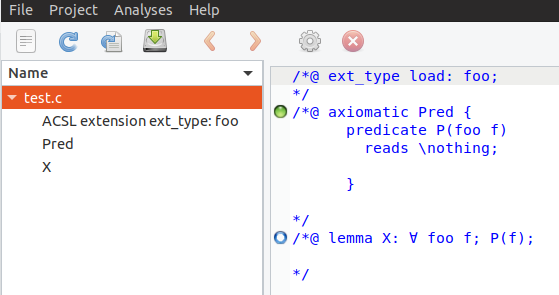
\includegraphics[width=\textwidth]{examples/acsl_extension_ext_types/acsl_extension_ext_types}



%%%%%%%%%%%%%%%%%%%%%%%%%%%%%%%%%%%%%%%%%%%%%%%%%%%%%%%%%%%%%%%%%%%%%%%%%%%%%%%

\section{Locations}\label{adv:memory}\index{Location|bfit}

\begin{prereq}
  None.
\end{prereq}

In \framac, different representations of \C locations
exist. Section~\ref{memory:repr} presents them. Moreover, maps indexed by
locations are also provided. Section~\ref{memory:map} introduces them.

\subsection{Representations}\label{memory:repr}

There are four different representations of \C locations. Actually only three
are really relevant. All of them are defined in module
\texttt{Locations}\codeidxdef{Locations}. They are introduced below. See the
documentation of \texttt{src/kernel\_services/abstract\_interp/locations.mli}
for details about the provided operations on these types.

\begin{itemize}
\item Type \texttt{Location\_Bytes.t}\scodeidxdef{Locations}{Location\_Bytes}
  is used to represent values of \C expressions like \texttt{2} or
  \texttt{((int) \&a) + 13}. With this representation, there is no way to know
  the size of a value while it is still possible to join two values. Roughly
  speaking it is represented by a mapping between \C variables and offsets in
  bytes.
\item Type \texttt{location}\scodeidxdef{Locations}{location}, equivalently
  \texttt{Location.t}\scodeidxdef{Locations}{Location} is used to represent the
  right part of a \C affectation (including bitfields). It is represented by a
  \texttt{Location\_Bits.t} (see below) attached to a size. It is possible to
  join two locations \emph{if and only if they have the same sizes.}
\item Type \texttt{Location\_Bits.t}\scodeidxdef{Locations}{Location\_Bits} is
  similar to \texttt{Location\_Bytes.t} with offsets in bits instead of
  bytes. Actually it should only be used inside a location.
\item Type \texttt{Zone.t}\scodeidx{Locations}{Zone} is a set of bits (without
  any specific order). It is possible to join two zones \emph{even if they have
    different sizes}.
\end{itemize}

\begin{convention}
  Roughly speaking, locations and zones have the same purpose. You should use
  locations as soon as you have no need to join locations of different sizes.
  If you require to convert locations to zones, use the function
  \texttt{Locations.enumerate\_valid\_bits}%
  \scodeidxdef{Locations}{enumerate\_valid\_bits}.
\end{convention}

As join operators are provided for these types, they can be easily used in
abstract interpretation analyses\index{Abstract Interpretation} (which can
themselves be implemented thanks to one of functors of module
\texttt{Dataflow2}\codeidx{Dataflow2}.

\subsection{Map Indexed by Locations}\label{memory:map}

Modules \texttt{Lmap}\codeidxdef{Lmap} and
\texttt{Lmap\_bitwise}\codeidxdef{Lmap\_bitwise} provide functors implementing
maps indexed by locations and zones (respectively). The argument of these
functors have to implement values attached to indices (resp. locations or zones).

These implementations are quite more complex than simple maps because they
automatically handle overlaps of locations (or zones). So such implementations
actually require that the structures implementing the values attached to indices
are at least semi-lattices\index{Lattice}; see the corresponding signatures
in module \texttt{Lattice\_type}\codeidx{Lattice\_type}. For
this purpose, functors of the abstract interpretation toolbox%
\index{Abstract Interpretation} can help (see in particular module
\texttt{Abstract\_interp}\codeidx{Abstract\_interp}).

%%%%%%%%%%%%%%%%%%%%%%%%%%%%%%%%%%%%%%%%%%%%%%%%%%%%%%%%%%%%%%%%%%%%%%%%%%%%%%%

\section{GUI Extension}\label{adv:gui}\index{GUI|bfit}\index{Plug-in!GUI|bfit}

\begin{prereq}
  Knowledge of \lablgtk.
\end{prereq}

Each plug-in can extend the \framac graphical user interface (aka \emph{GUI})
in order to support its own functionalities in the \framac viewer. For this
purpose, a plug-in developer has to register a function of type
\texttt{Design.main\_window\_extension\_points \fl~unit} thanks to
\texttt{Design.register\_extension}\scodeidx{Design}{register\_extension}. The
input value of type \texttt{Design.main\_window\_extension\_points} is an
object corresponding to the main window of the \framac GUI. It provides
accesses to the main widgets of the \framac GUI and to several plug-in extension
points. The documentation of the class type
\texttt{Design.main\_window\_extension\_points}%
\scodeidxdef{Design}{main\_window\_extension\_points} is accessible through the
source documentation (see Section~\ref{tut2:doc}).

Besides time-consuming computations have to call the function
\texttt{Async.yield}\scodeidx{Async}{yield} from time to time in order to keep the GUI reactive.

%Mainly that's all!
The GUI implementation uses
\lablgtk~\cite{lablgtk}\index{Lablgtk}: you can use any \lablgtk-compatible
code in your gui extension. A complete example of a GUI extension may be found in
the plug-in \texttt{Occurrence}\index{Occurrence} (see file
\texttt{src/plugins/occurrence/gui/register\_gui.ml}).

\begin{important}
\paragraph{Potential issues}
All the GUI plug-in extensions share the same window and same
widgets\index{Sharing!Widget}. So conflicts can occur, especially if you
specify some attributes on a predefined object. For example, if a plug-in wants
to highlight\index{Highlighting} a statement $s$ in yellow and another one
wants to highlight $s$ in red at the same time, the behavior is not specified
but it could be quite difficult to understand for an user.
\end{important}

%%%%%%%%%%%%%%%%%%%%%%%%%%%%%%%%%%%%%%%%%%%%%%%%%%%%%%%%%%%%%%%%%%%%%%%%%%%%%%%

% \section{Documentation}\label{adv:documentation}
% \index{Documentation|bfit}

% \begin{prereq}
%   Knowledge of \odoc.
% \end{prereq}

% Here we present some hints on the way to document your plug-in. First
% Section~\ref{doc:rules} introduces a quick general overview about the
% documentation process. Next Section~\ref{doc:plugin} focuses on the
% plug-in source documentation.

% \subsection{General Overview}\label{doc:rules}

% Command \texttt{make doc}\codeidx{Makefile} produces the whole \framac source
% documentation\index{Documentation!Source} in HTML format. The generated index
% file is \texttt{doc/code/html/index.html}. A more general purpose index is
% \texttt{doc/index.html}\codeidx{index.html} (from which the previous index is
% accessible).

% The previous command takes times. So command \texttt{make doc-kernel} only
% generates the kernel documentation\index{Documentation!Kernel} (\emph{i.e.}
% \framac without any plug-in) while \texttt{make \$(PLUGIN\_NAME)\_DOC} (by
% substituting the right value for
% \texttt{\$(PLUGIN\_NAME)})\codeidx{PLUGIN\_NAME} generates
% the documentation for a single plug-in\index{Plug-in!Documentation}%
% \index{Documentation!Plug-in|see{Plug-in Documentation}}.

% \subsection{Source Documentation}\label{doc:plugin}
% \index{Plug-in!Documentation|bfit}

% Each plug-in should be properly documented. \framac uses \ocamldoc and so you
% can write any valid \ocamldoc comments.

% \paragraph{\ocamldoc tags for \framac}\index{Documentation!Tags} The tag
% \texttt{@since version} should document any element introduced after the very
% first release, in order to easily know the required version of the \framac
% kernel or specific plug-ins. In the same way, the \framac documentation
% generator provides a custom tag \texttt{@modify version description} which
% should be used to document any element which semantics have changed since its
% introduction.

% Furthermore, the special tag \texttt{@plugin developer guide} must be attached
% to each function used in this document.

% \paragraph{Plug-in API}

% A plug-in should export functions in its plug-in interface or through modules
% \texttt{Db}\codeidx{Db} or \texttt{Dynamic}\codeidx{Dynamic} as explained in
% Section~\ref{adv:plugin-registration}.

% \begin{important}
% The interface name of a plug-in \texttt{plugin} must be \texttt{Plugin.mli}. Be
% careful to capitalization of the filename which is unusual in \caml but
% required here for compilation purposes.
% \end{important}

% \paragraph{Internal Documentation for Kernel Integrated Plug-ins}

% The \framac documentation generator also produces an internal plug-in
% documentation which may be useful for the plug-in developer itself.

% \paragraph{Internal Documentation for External Plug-ins}

% External plug-ins can be documented in the same way as plug-ins that are
% compiled together with \framac. However, in order to be able to compile the
% documentation with \texttt{make doc}, you must have generated the documentation
% of Frama-C's kernel (\texttt{make doc}, see above) and installed it with the
% \texttt{make install-doc-code}\codeidx{install-doc-code} command.

\section{Packaging}
\label{sec:dune-packaging}

If you intend to release your plug-in, a possible way is to take advantage of
the \texttt{opam} integration within
\texttt{dune}\footnote{\url{https://dune.readthedocs.io/en/stable/opam.html}}.
Basically, the \index{dune-project}\texttt{dune-project} file
(see Section~\ref{tut2:hello}) should contain a stanza
\texttt{(generate\_opam\_files true)}, as well as some meta-information
(location of the sources, licence, author(s), etc.). It is also possible to
provide this information in a file \texttt{my-plugin-package.opam.template},
assuming \texttt{my-plugin-package} is the name of the package of the plug-in in
the \texttt{dune-project} file. See the dune documentation for detailed information
about the creation of the \texttt{opam} file.

\section{Profiling with Landmarks} \label{refman:landmarks}\codeidxdef{Landmarks}

{\em Landmarks}\footnote{\url{https://github.com/LexiFi/landmarks}} is a
library for ``quick and dirty'' profiling of OCaml programs. It allows the
insertion of annotations in the code to enable profiling of specific parts of
it, but also an automatic mode, in which every function call is instrumented.
This can help quickly obtain some profiling data for a plug-in or a specific
test case.

For quick usage of the library:
\begin{itemize}
\item make sure that you have packages \texttt{landmarks} and
  \texttt{landmarks-ppx} installed;
\item run \texttt{make DUNE\_WS=bench} to compile \framac using
  \texttt{dev/dune-workspace.bench}, which sets up a specific {\em Dune context}
  to enable instrumentation without affecting the default context.
  This compiles each \framac file in a different directory inside
  \texttt{\_build}.
\item install the instrumented \framac: \texttt{make install DUNE\_WS=bench}.
\item enable instrumentation {\em during execution} of \framac, using the
  \texttt{OCAML\_LANDMARKS} environment variable:
\begin{logs}
OCAML_LANDMARKS=<options> frama-c [files] [options]
\end{logs}
  The easiest setup is \texttt{OCAML\_LANDMARKS=auto}, which will instrument
  everything and output timing information to \texttt{stderr} after
  program termination.
  You can also use \texttt{OCAML\_LANDMARKS=auto,output=landmarks.log} to
  output the timing information to file \texttt{landmarks.log}.
\item you can also run the instrumented \framac without installing it, via
  \texttt{dune exec}:
\begin{logs}
OCAML_LANDMARKS=auto dune exec --workspace dev/dune-workspace.bench \
  --context bench -- frama-c [files] [options]
\end{logs}
  The \verb+--workspace dev/dune-workspace.bench+ argument tells Dune to use
  the workspace in which Landmarks is configured.

  The \verb+--context bench+ argument tells Dune to use the instrumented
  context. This context is different from the default one in order to avoid
  overwriting non-instrumented files when running \texttt{make} without
  \texttt{DUNE\_WS}.
\end{itemize}

To instrument a single file: add \verb+[@@@landmark "auto"]+ at the beginning
of the file.

To instrument a single function: add \verb+[@landmark]+ after the \texttt{let},
e.g.:

\begin{ocamlcode}
  let[@landmark] add_visitor vis =
\end{ocamlcode}

Check \url{https://github.com/LexiFi/landmarks} for its documentation.

\section{Profiling a custom plug-in}

To profile your own plug-in using Landmarks, do the following:

\begin{enumerate}
\item Add \verb|(instrumentation (backend landmarks))| to your plug-in's
  \verb|dune| file, inside the \verb|library| stanza, as in the example below:
\begin{dunecode}
 (library
   (name my-plug-in)
   (public_name frama-c-my-plug-in.core)
   ...
   (libraries frama-c.kernel)
   (instrumentation (backend landmarks)) ; <<< ADD THIS LINE
 )
\end{dunecode}
\item Create a \verb|dune-workspace.bench| file in your plugin's top-level
  directory:
  \listingname{dune-workspace.bench}
  \duneinput{dune-workspace.bench}
\item Add \verb|--workspace=dune-workspace.bench| to the \verb|dune build|
  and \verb|dune install| commands that you run, e.g.:
\begin{logs}
dune build --workspace=dune-workspace.bench @install
dune install --workspace=dune-workspace.bench
\end{logs}
This will compile and install the plug-in with Landmarks instrumentation
enabled. Then you just need to set \verb|OCAML_LANDMARKS| as described in the
previous section, e.g.:
\begin{logs}
OCAML_LANDMARKS=auto frama-c [my-plugin-options]
\end{logs}
\item For \verb|dune exec|, you need to add the \verb|--workspace| option
  as well as \verb|--context bench|. Combined with \verb|OCAML_LANDMARKS|,
  the command-line will resemble the following:
\begin{logs}
OCAML_LANDMARKS=auto dune exec --workspace dev/dune-workspace.bench \
  --context bench -- frama-c [files] [options]
\end{logs}
\end{enumerate}
